\documentclass[xcolor={table}]{beamer}
\usepackage{fleqn}
\usepackage{graphicx}
\usepackage{coordsys} %for \numbline commander

%Setup appearance:
\usetheme{Darmstadt}
\usefonttheme[onlylarge]{structurebold}
\setbeamerfont*{frametitle}{size=\normalsize,series=\bfseries}
\setbeamertemplate{navigation symbols}{}
\setbeamertemplate{bibliography item}{[\theenumiv]}

% Standard packages
\usepackage[english]{babel}
\usepackage[latin1]{inputenc}
\usepackage{times}
\usepackage[T1]{fontenc}
\usepackage{multirow}
\usepackage{subfigure}
\usepackage{pbox}
\usepackage{arydshln}
\usepackage{pifont}
\usepackage{cancel}
\usepackage{rotating} % for sideways headings

% Source Code packages
\usepackage{algorithm2e}
\usepackage{algorithmic}

\DeclareSymbolFont{extraup}{U}{zavm}{m}{n}
\DeclareMathSymbol{\varclub}{\mathalpha}{extraup}{84}
\DeclareMathSymbol{\varspade}{\mathalpha}{extraup}{85}
\DeclareMathSymbol{\varheart}{\mathalpha}{extraup}{86}
\DeclareMathSymbol{\vardiamond}{\mathalpha}{extraup}{87}

%%% This section command that adds a big page with section dividers
\usepackage{xifthen}% provides \isempty test
\newcommand{\SectionSlide}[2][]{
	\ifthenelse{\isempty{#1}}
		{\section{#2}\begin{frame} \begin{center}\begin{huge}#2\end{huge}\end{center}\end{frame}}
		{\section[#1]{#2}\begin{frame} \begin{center}\begin{huge}#2\end{huge}\end{center}\end{frame}}
}
%Extends the section slide to to include a shortened section title for the navigation bar as a second parameter
\newcommand{\SectionSlideShortHeader}[3][]{
	\ifthenelse{\isempty{#1}}
		{\section[#3]{#2}\begin{frame} \begin{center}\begin{huge}#2\end{huge}\end{center}\end{frame}}
		{\section[#1]{#2}\begin{frame} \begin{center}\begin{huge}#3\end{huge}\end{center}\end{frame}}
}

\newcommand{\refer}[1]{\footnote{#1}}
\newcommand{\GW}{\text{\textit{Guess-Who~}}}
\newcommand{\keyword}[1]{\alert{\textbf{#1}}\index{#1}}
\newcommand{\firstkeyword}[1]{\textbf{#1}\index{#1}}
\newcommand{\indexkeyword}[1]{\alert{\textbf{#1}\index{#1}}}
\newcommand{\featN}[1]{\textsc{#1}}
\newcommand{\featL}[1]{\textit{'#1'}}
 \newcommand{\ourRef}[1]{\ref{#1} $^{\text{\tiny[\pageref{#1}]}}$}
 \newcommand{\ourEqRef}[1]{\eqref{#1}$^{\text{\tiny[\pageref{#1}]}}$}
  
\DeclareMathOperator*{\argmax}{argmax}
\DeclareMathOperator*{\argmin}{argmin}



\title{Evaluation\\Sections $9.4, 9.5$}
	\author{John D. Kelleher and Brian Mac Namee and Aoife D'Arcy}
	\institute{}
	\date{}
\begin{document}
\begin{frame}
	\titlepage
\end{frame}

\begin{frame}[plain]
	\begin{scriptsize}
	\vspace{0.25cm}
	\tableofcontents
	\end{scriptsize}
\end{frame}


\SectionSlideShortHeader{Designing Evaluation Experiments}{Design}

\subsection{Hold-out Sampling}

 \begin{frame} 
\begin{figure}[htb]
       \begin{centering}
			\subfigure[A $50$:$20$:$30$ split]{\includegraphics[width=0.65\textwidth]{images/EvaluationProcessesTrainValidTest1.pdf}}
			\subfigure[A $40$:$20$:$40$ split]{\includegraphics[width=0.65\textwidth]{images/EvaluationProcessesTrainValidTest2.pdf}}
       \caption{\indexkeyword{Hold-out sampling} can divide the full data into training, validation, and test sets.}
       \label{fig:holdoutTestTrainingValidation}
       \end{centering}
\end{figure}
\end{frame} 

 \begin{frame} 
\begin{figure}[htb]
       \begin{centering}
			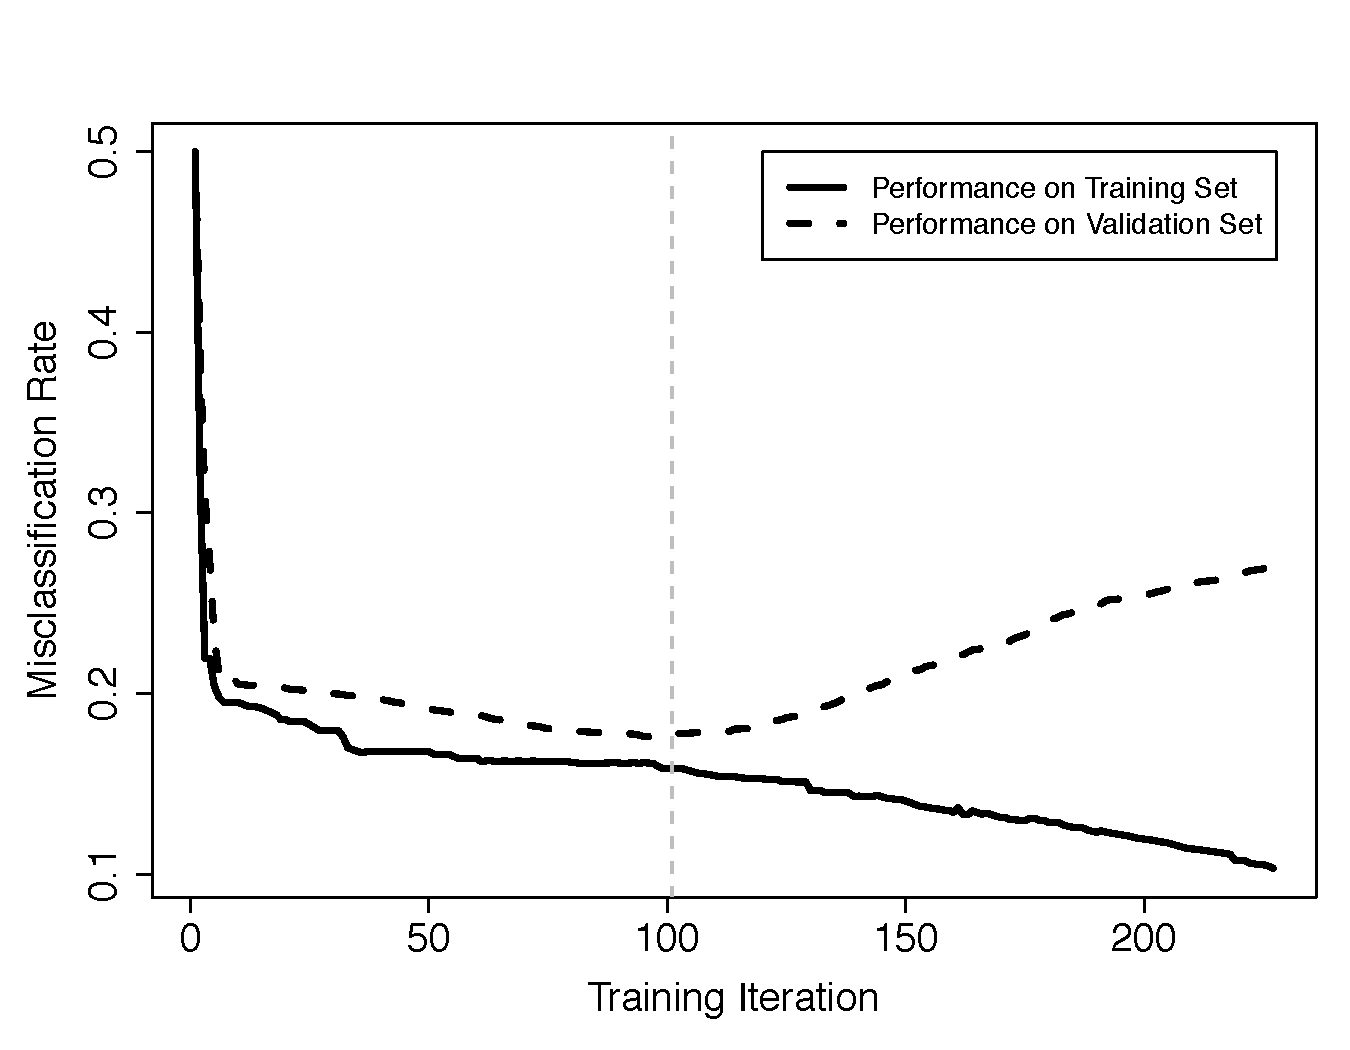
\includegraphics[width=0.54\linewidth]{images/InformationBased-ChurnIterationPlotRevised.pdf}
       \caption{Using a validation set to avoid overfitting in iterative machine learning algorithms.}
       \label{fig:avoidOverfittingTrainVValidn}
       \end{centering}
\end{figure}
\end{frame} 

\subsection{k-Fold Cross Validation}

 \begin{frame}[plain]
\begin{table}[!thb]
\centering
\begin{tiny}
\begin{tabular}{c c c}
\hline
Fold & Confusion Matrix & \pbox{20cm}{Class \\ Accuracy} \\
\hline
~ & ~ & ~ \\
1 & 
{\begin{tabular}{c >{}r @{\hspace{0.7em}} | c @{\hspace{0.4em}} c @{\hspace{0.7em}}}
    & &  \multicolumn{2}{c}{Prediction} \\
  & & \featL{lateral} & \featL{frontal}  \\
  \hline
  \multirow{2}{*}{\parbox{1.1cm}{\raggedleft Target}}  & \featL{lateral} & $43$	&	$9$ \\
  & \featL{frontal} & $10$	&	$38$
\end{tabular}
} 
& $81\%$ \\
~ & ~ & ~ \\
2 & 
{\begin{tabular}{c >{}r @{\hspace{0.7em}} | c @{\hspace{0.4em}} c @{\hspace{0.7em}}}
    & &  \multicolumn{2}{c}{ Prediction} \\
  & &  \featL{lateral} &  \featL{frontal}  \\
  \hline
  \multirow{2}{*}{\parbox{1.1cm}{\raggedleft Target}}  & \featL{lateral} & $46$	&	$9$ \\
  & \featL{frontal} & $3$	&	$42$
\end{tabular}
} 
& $88\%$ \\
~ & ~ & ~ \\
3 & 
{\begin{tabular}{c >{}r @{\hspace{0.7em}} | c @{\hspace{0.4em}} c @{\hspace{0.7em}}}
    & &  \multicolumn{2}{c}{ Prediction} \\
  & &  \featL{lateral} &  \featL{frontal}  \\
  \hline
  \multirow{2}{*}{\parbox{1.1cm}{\raggedleft Target}}  & \featL{lateral} & $51$	&	$10$ \\
  & \featL{frontal} & $8$	&	$31$
\end{tabular}
} 
& $82\%$ \\
~ & ~ & ~ \\ 
4 & 
{\begin{tabular}{c >{}r @{\hspace{0.7em}} | c @{\hspace{0.4em}} c @{\hspace{0.7em}}}
    & &  \multicolumn{2}{c}{ Prediction} \\
  & &  \featL{lateral} &  \featL{frontal}  \\
  \hline
  \multirow{2}{*}{\parbox{1.1cm}{\raggedleft Target}}  & \featL{lateral} & $51$	&	$8$ \\
  & \featL{frontal} & $7$	&	$34$
\end{tabular}
} 
& $85\%$ \\
~ & ~ & ~ \\
5 & 
{\begin{tabular}{c >{}r @{\hspace{0.7em}} | c @{\hspace{0.4em}} c @{\hspace{0.7em}}}
    & &  \multicolumn{2}{c}{ Prediction} \\
  & &  \featL{lateral} &  \featL{frontal}  \\
  \hline
  \multirow{2}{*}{\parbox{1.1cm}{\raggedleft Target}}  & \featL{lateral} & $46$	&	$9$ \\
  & \featL{frontal} & $7$	&	$38$
\end{tabular}
} 
& $84\%$ \\
~ & ~ & ~ \\
\hline
~ & ~ & ~ \\
Overall & 
{\begin{tabular}{c >{}r @{\hspace{0.7em}} | c @{\hspace{0.4em}} c @{\hspace{0.7em}}}
    & &  \multicolumn{2}{c}{ Prediction} \\
  & &  \featL{lateral} &  \featL{frontal}  \\
  \hline
  \multirow{2}{*}{\parbox{1.1cm}{\raggedleft Target}}  & \featL{lateral} & $237$	&	$45$ \\
  & \featL{frontal} & $35$	&	$183$
\end{tabular}
} 
& $84\%$ \\
\end{tabular}
\end{tiny}
\end{table}
\end{frame} 

 \begin{frame} 
\begin{figure}[htb]
       \begin{centering}
			\includegraphics[width=0.85\textwidth]{images/EvaluationProcessesKFold.pdf}
       \caption{The division of data during the \indexkeyword{\textit{k}-fold cross validation} process. Black rectangles indicate test data, and white spaces indicate training data.}
       \label{fig:kFoldCrossValidation}
       \end{centering}
\end{figure}
\end{frame} 

\subsection{Leave-one-out Cross Validation}

 \begin{frame} 
\begin{figure}[htb]
       \begin{centering}
			\includegraphics[width=0.85\textwidth]{images/EvaluationProcessesLeaveOneOut2.pdf}
       \caption{The division of data during the \indexkeyword{leave-one-out cross validation} process. Black rectangles indicate instances in the test set, and white spaces indicate training data.}
       \label{fig:looCrossValidation}
       \end{centering}
\end{figure}
\end{frame} 

\subsection{Bootstrapping}

 \begin{frame} 
\begin{figure}[htb]
       \begin{centering}
			\includegraphics[width=0.85\textwidth]{images/EvaluationProcessesBootstrap.pdf}
       \caption{The division of data during the $\epsilon0$ bootstrap process. Black rectangles indicate test data, and white spaces indicate training data.}
       \label{fig:bootstrapping}
       \end{centering}
\end{figure}
\end{frame} 

\subsection{Out-of-time Sampling}

 \begin{frame} 
\begin{figure}[htb]
       \begin{centering}
			\includegraphics[width=0.75\textwidth]{images/EvaluationProcessesOutOfTime.pdf}
       \caption{The \indexkeyword{out-of-time sampling} process.}
       \label{fig:outOfTimeSampling}
       \end{centering}
\end{figure}
\end{frame} 


\SectionSlideShortHeader{Performance Measures: Categorical Targets}{Cat. Targets}

\subsection{Confusion Matrix-based Performance Measures}

 \begin{frame} 
\begin{alignat}{2}
\text{TPR} & = \frac{TP}{\left(TP + FN\right)} \label{eqn:tpr}\\
\text{TNR} & = \frac{TN}{\left(TN + FP\right)}  \label{eqn:tnr} \\
\text{FPR} & = \frac{FP}{\left(TN + FP\right)}  \label{eqn:fpr} \\
\text{FNR} & = \frac{FN}{\left(TP + FN\right)}  \label{eqn:fnr} 
\end{alignat}
\end{frame} 

 \begin{frame} 
\begin{eqnarray*}
\text{TPR} & = \frac{6}{\left(6 + 3\right)} & = 0.667 \\
\text{TNR} & = \frac{9}{\left(9 + 2\right)} & = 0.818 \\
 \text{FPR} & = \frac{2}{\left(9 + 2\right)} & = 0.182 \\
 \text{FNR} & = \frac{3}{\left(6 + 3\right)} & = 0.333 
\end{eqnarray*} 
\end{frame} 

\subsection{Precision, Recall and F$_1$ Measure}

 \begin{frame} 
\begin{alignat}{2}
\text{precision} & = \frac{TP}{\left(TP + FP\right)} \label{eqn:precision}\\
\text{recall} & = \frac{TP}{\left(TP + FN\right)}  \label{eqn:recall}
\end{alignat}
\end{frame} 

 \begin{frame} 
\begin{alignat*}{2}
\text{precision} & = \frac{6}{\left(6 + 2\right)} & = 0.75 \\
\text{recall} & = \frac{6}{\left(6 + 3\right)} & = 0.667
\end{alignat*}
\end{frame} 

 \begin{frame} 
\begin{alignat}{2}
\text{F$_1$-measure} & = 2 \times \frac{\left(\text{precision} \times \text{recall} \right)}{\left(\text{precision} + \text{recall}\right)}
\label{eqn:f1Measure}
\end{alignat}
\pause
\begin{alignat*}{2}
\text{F$_1$-measure} & = 2 \times \frac{\left(\frac{6}{\left(6 + 2\right)} \times  \frac{6}{\left(6 + 3\right)} \right)}{\left(\frac{6}{\left(6 + 2\right)} +  \frac{6}{\left(6 + 3\right)} \right)} \\
 & = 0.706
\end{alignat*}
\end{frame} 

\subsection{Average Class Accuracy}

 \begin{frame} 
\begin{table}
\caption{A confusion matrix for a $k$-NN model trained on a churn prediction problem.}
\label{tab:imbalancedConfusionMatrices1}
\centering
\begin{footnotesize}
\begin{tabular}{c >{\bfseries}r @{\hspace{0.7em}} | c @{\hspace{0.4em}} c @{\hspace{0.7em}}}
    & &  \multicolumn{2}{c }{\bfseries Prediction}  \\
  & & \bfseries \featL{non-churn} & \bfseries \featL{churn} \\
  \hline
  \multirow{2}{*}{\parbox{1.1cm}{\bfseries\raggedleft Target}}  & \featL{non-churn} & $90$	&	$0$ \\
  & \featL{churn} & $9$	&	$1$ \\
\end{tabular}
\end{footnotesize}
\end{table}
\begin{table}
\caption{A confusion matrix for a naive Bayes model trained on a churn prediction problem.}
\label{tab:imbalancedConfusionMatrices2}
\centering
\begin{footnotesize}
\begin{tabular}{c >{\bfseries}r @{\hspace{0.7em}} | c @{\hspace{0.4em}} c @{\hspace{0.7em}}}
    & &  \multicolumn{2}{c }{\bfseries Prediction}\\
  & & \bfseries \featL{non-churn} & \bfseries \featL{churn} \\
  \hline
  \multirow{2}{*}{\parbox{1.1cm}{\bfseries\raggedleft Target}}  & \featL{non-churn} & $70$	&	$20$  \\
  & \featL{churn} & $2$	&	$8$\\
\end{tabular}
\end{footnotesize}
\end{table}
\end{frame} 



 \begin{frame} 
\begin{equation}
\text{average class accuracy}=\frac{1}{|levels(t)|}\sum_{l \in levels(t)} \text{recall}_l
\label{eq:averageClassAccuracyArithmetic}
\end{equation}
\end{frame} 

 \begin{frame} 
\begin{alignat}{2}
\text{average class accuracy}_\text{HM}= \displaystyle \frac{1}{\displaystyle \frac{1}{|levels(t)|}\sum_{l \in levels(t)} \frac{1}{\text{recall}_l}}
\label{eq:averageClassAccuracyHarmonic}
\end{alignat}
\end{frame} 

 \begin{frame} 
\begin{alignat*}{2}
\displaystyle \frac{1}{\displaystyle \frac{1}{2}\left(\frac{1}{1.0} + \frac{1}{0.1}\right)} = \frac{1}{5.5} = 18.2\%
\end{alignat*}
\begin{alignat*}{2}
\displaystyle \frac{1}{\displaystyle \frac{1}{2}\left(\frac{1}{0.778} + \frac{1}{0.800}\right)} = \frac{1}{1.268} = 78.873\%
\end{alignat*}
\end{frame} 

 \begin{frame} 
\begin{figure}[htb]
       \begin{centering}
			\subfigure[]{\label{fig:meansDemoArithmetic}\includegraphics[width=0.45\textwidth]{images/EvaluationMeansDemo-Arithmetic3.png}}
			\subfigure[]{\label{fig:meansDemoHarmonic}\includegraphics[width=0.45\textwidth]{images/EvaluationMeansDemo-Harmonic3.png}}
       \caption{Surfaces generated by calculating (a) the \indexkeyword{arithmetic mean} and (b) the \indexkeyword{harmonic mean} of all combinations of features A and B that range from $0$ to $100$.}
       \label{fig:meansDemo}
       \end{centering}
\end{figure}
\end{frame} 

\subsection{Measuring Profit and Loss}

 \begin{frame} 
  \begin{itemize}
 	\item It is not always correct to treat all outcomes equally
	\item In these cases, it is useful to take into account the cost of the different outcomes when evaluating models
\end{itemize}
\end{frame}

\begin{frame}
\begin{table}
\caption{The structure of a \indexkeyword{profit matrix}.}
\label{tab:profitMatrixStucture}
\center
\begin{footnotesize}
\begin{tabular}{c >{\bfseries}r @{\hspace{0.7em}} | c @{\hspace{0.4em}} c @{\hspace{0.7em}}}
    & &  \multicolumn{2}{c}{\bfseries Prediction} \\
  & & \bfseries positive & \bfseries negative  \\
  \hline
  \multirow{2}{*}{\parbox{1.1cm}{\bfseries\raggedleft Target}}  & positive & $TP_{\text{Profit}}$	&	$FN_{\text{Profit}}$ \\
  & negative & $FP_{\text{Profit}}$	&	$TN_{\text{Profit}}$
\end{tabular}
\end{footnotesize}
\end{table}
\end{frame} 

 \begin{frame} 
\begin{table}[htb]
\caption{The \indexkeyword{profit matrix} for the pay-day loan credit scoring problem.}
\label{tab:profitMatrixExample}
\centering
\begin{footnotesize}
\begin{tabular}{c >{\bfseries}r @{\hspace{0.7em}} | r @{\hspace{0.4em}} r @{\hspace{0.7em}}}
    & &  \multicolumn{2}{c}{\bfseries Prediction} \\
  & & \bfseries \featL{good} & \bfseries \featL{bad}  \\
  \hline
  \multirow{2}{*}{\parbox{1.1cm}{\bfseries\raggedleft Target}}  & \featL{good} & $140$	&	$-140$ \\
  & \featL{bad} & $-700$	&	$0$
\end{tabular}
\end{footnotesize}
\end{table}
\end{frame} 

 \begin{frame} 
\begin{table}
\caption{(a) The confusion matrix for a $k$-NN model trained on the pay-day loan credit scoring problem ($\text{average class accuracy}_{HM} = 83.824\%$); (b) the confusion matrix for a decision tree model trained on the pay-day loan credit scoring problem ($\text{average class accuracy}_{HM} = 80.761\%$).}
\label{tab:profitMatrixExampleCM}
\centering
\begin{footnotesize}
\subtable[$k$-NN model]{\label{tab:profitMatrixExampleCM1}\begin{tabular}{c >{\bfseries}r @{\hspace{0.7em}} | c @{\hspace{0.4em}} c @{\hspace{0.7em}} }
    & &  \multicolumn{2}{c }{\bfseries Prediction} \\
  & & \bfseries \featL{good} & \bfseries \featL{bad} \\
  \hline
  \multirow{2}{*}{\parbox{1.1cm}{\bfseries\raggedleft Target}}  & \featL{good} & $57$	&	$3$ \\
  & \featL{bad} & $10$	&	$30$ \\
\end{tabular}}
\subtable[decision tree]{\label{tab:profitMatrixExampleCM2}\begin{tabular}{c >{\bfseries}r @{\hspace{0.7em}} | c @{\hspace{0.4em}} c @{\hspace{0.7em}} }
    & &  \multicolumn{2}{c }{\bfseries Prediction} \\
  & & \bfseries \featL{good} & \bfseries \featL{bad} \\
  \hline
  \multirow{2}{*}{\parbox{1.1cm}{\bfseries\raggedleft Target}}  & \featL{good} & $43$	&	$17$ \\
  & \featL{bad} & $3$	&	$37$ \\
\end{tabular}}
\end{footnotesize}
\end{table}
\end{frame} 

 \begin{frame} 
\begin{table}
\caption{(a) Overall profit for the $k$-NN model using the profit matrix in Table \ourRef{tab:profitMatrixExample} and the \indexkeyword{confusion matrix} in Table \ourRef{tab:profitMatrixExampleCM1}; (b) overall profit for the decision tree model using the profit matrix in Table \ourRef{tab:profitMatrixExample} and the \indexkeyword{confusion matrix} in Table \ourRef{tab:profitMatrixExampleCM2}.}
\label{tab:profitMatrixExampleSum}
\centering
\begin{footnotesize}
\subtable[$k$-NN model]{\label{tab:profitMatrixExampleSum1}\begin{tabular}{c >{\bfseries}r @{\hspace{0.7em}} | r @{\hspace{0.4em}} r @{\hspace{0.7em}}}
    & &  \multicolumn{2}{c}{\bfseries Prediction} \\
  & & \bfseries \featL{good} & \bfseries \featL{bad} \\
  \hline
  \multirow{2}{*}{\parbox{1.1cm}{\bfseries\raggedleft Target}}  & \featL{good} & $7\,980$	&	$-420$\\
  & \featL{bad} & $-7\,000$	&	$0$\\
  \hline
  & \textbf{Profit} &  \multicolumn{2}{|r}{$\textbf{560}$} 
\end{tabular}}
\subtable[decision tree]{\label{tab:profitMatrixExampleSum2}\begin{tabular}{c >{\bfseries}r @{\hspace{0.7em}} | r @{\hspace{0.4em}} r @{\hspace{0.7em}}}
    & &  \multicolumn{2}{c}{\bfseries Prediction} \\
  & & \bfseries \featL{good} & \bfseries \featL{bad} \\
  \hline
  \multirow{2}{*}{\parbox{1.1cm}{\bfseries\raggedleft Target}}  & \featL{good} & $6\,020$	&	$-2\,380$\\
  & \featL{bad} & $-2\,100$	&	$0$\\
  \hline
  & \textbf{Profit} &  \multicolumn{2}{|r}{$\textbf{1\,540}$} 
\end{tabular}}
\end{footnotesize}
\end{table}
\end{frame} 

\SectionSlideShortHeader{Performance Measures: Prediction Scores}{Pred. Scores}

 \begin{frame} 
 \begin{itemize}
 	\item All our classification prediction models return a score which is then thresholded.
\end{itemize}
 \begin{example}
\begin{alignat}{2}
threshold(score, 0.5) = \begin{cases}
		positive & \text{if } score \ge 0.5\\
		negative & otherwise
	\end{cases}
\end{alignat}
\end{example}
\end{frame} 

 \begin{frame} 
\begin{table}[htb]
\caption{A sample test set with model predictions and scores (threshold$=0.5$.}
\label{tab:samplePredictionExampleExtended}
\centering
\begin{tiny}
\begin{tabular}{cc}
		\hline
			\begin{minipage}{0.45\textwidth}
						\centering
					\begin{tabular}{  c  c  c  c  c }
~	 & ~	& Pred- & ~ & Out-\\
\featN{ID}	 & Target	& iction & Score & come\\
\hline
7	&	ham	&	ham	&	0.001	&	TN	\\
11	&	ham	&	ham	&	0.003	&	TN	\\
15	&	ham	&	ham	&	0.059	&	TN	\\
13	&	ham	&	ham	&	0.064	&	TN	\\
19	&	ham	&	ham	&	0.094	&	TN	\\
12	&	spam	&	ham	&	0.160	&	FN	\\
2	&	spam	&	ham	&	0.184	&	FN	\\
3	&	ham	&	ham	&	0.226	&	TN	\\
16	&	ham	&	ham	&	0.246	&	TN	\\
1	&	spam	&	ham	&	0.293	&	FN	\\
\hline 
\end{tabular}
			\end{minipage}
			&
			\begin{minipage}{0.45\textwidth}
			\centering
										\begin{tabular}{  c  c  c  c  c }
~	 & ~	& Pred- & ~ & Out-\\
\featN{ID}	 & Target	& iction & Score & come\\
\hline
5	&	ham	&	ham	&	0.302	&	TN	\\
14	&	ham	&	ham	&	0.348	&	TN	\\
17	&	ham	&	spam	&	0.657	&	FP	\\
8	&	spam	&	spam	&	0.676	&	TP	\\
6	&	spam	&	spam	&	0.719	&	TP	\\
10	&	spam	&	spam	&	0.781	&	TP	\\
18	&	spam	&	spam	&	0.833	&	TP	\\
20	&	ham	&	spam	&	0.877	&	FP	\\
9	&	spam	&	spam	&	0.960	&	TP	\\
4	&	spam	&	spam	&	0.963	&	TP	\\
\hline 
\end{tabular}
			\end{minipage}
\end{tabular}
\end{tiny}
\end{table}
\end{frame} 

\begin{frame}
	\begin{itemize}
		\item We have ordered the examples by score so the threshold is apparent in the predictions.
		\item Note that, in general, instances that actually should get a prediction of \featL{ham} generally have a low score, and those that should get a prediction of \featL{spam} generally get a high score.
	\end{itemize}
\end{frame}

\begin{frame}
	\begin{itemize}
		\item There are a number of performance measures that use this ability of a model to rank instances that should get predictions of one target level higher than the other, to assess how well the model is performing.
		\item The basis of most of these approaches is measuring \alert{how well the distributions of scores produced by the model for different target levels are separated}
	\end{itemize}
\end{frame}

 \begin{frame} 
\begin{figure}[htb]
       \begin{centering}
			\subfigure[]{\label{fig:scoreDistributions1}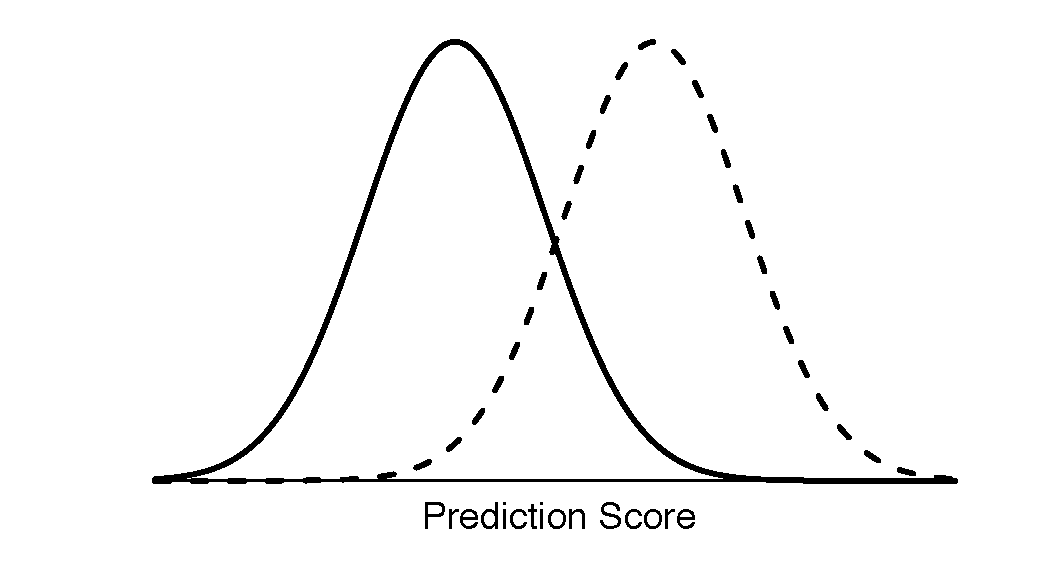
\includegraphics[width=0.45\textwidth]{images/classification_score_dist_1.pdf}}
			\subfigure[]{\label{fig:scoreDistributions2}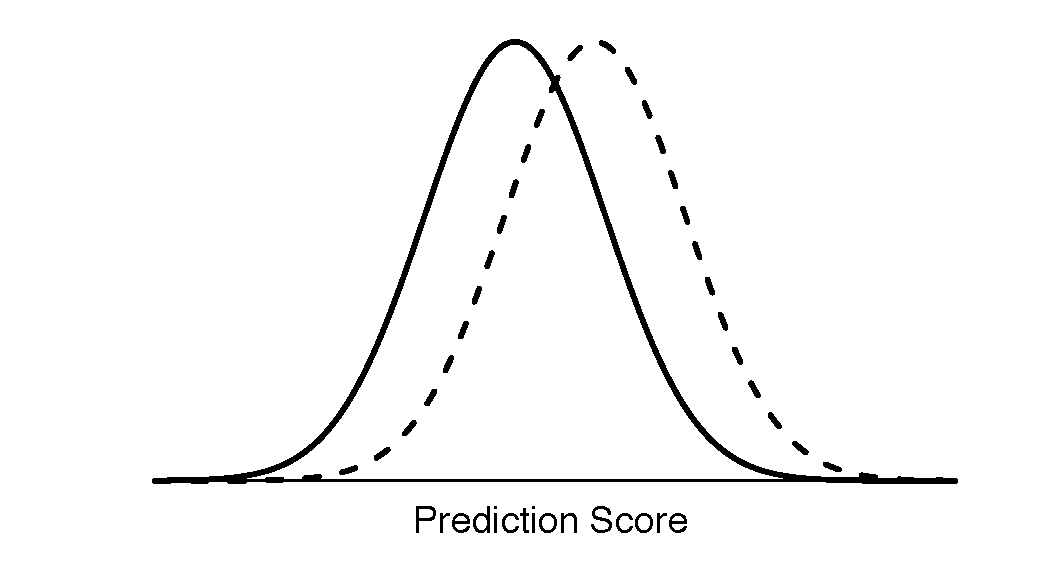
\includegraphics[width=0.45\textwidth]{images/classification_score_dist_2.pdf}}
       \caption{Prediction score distributions for two different prediction models. The distributions in (a) are much better separated than those in (b).}
       \label{fig:scoreDistributions}
       \end{centering}
\end{figure}
\end{frame} 

 \begin{frame} 
\begin{figure}[htb]
       \begin{centering}
			\subfigure[spam]{\label{fig:scoreExampleHistosSpam}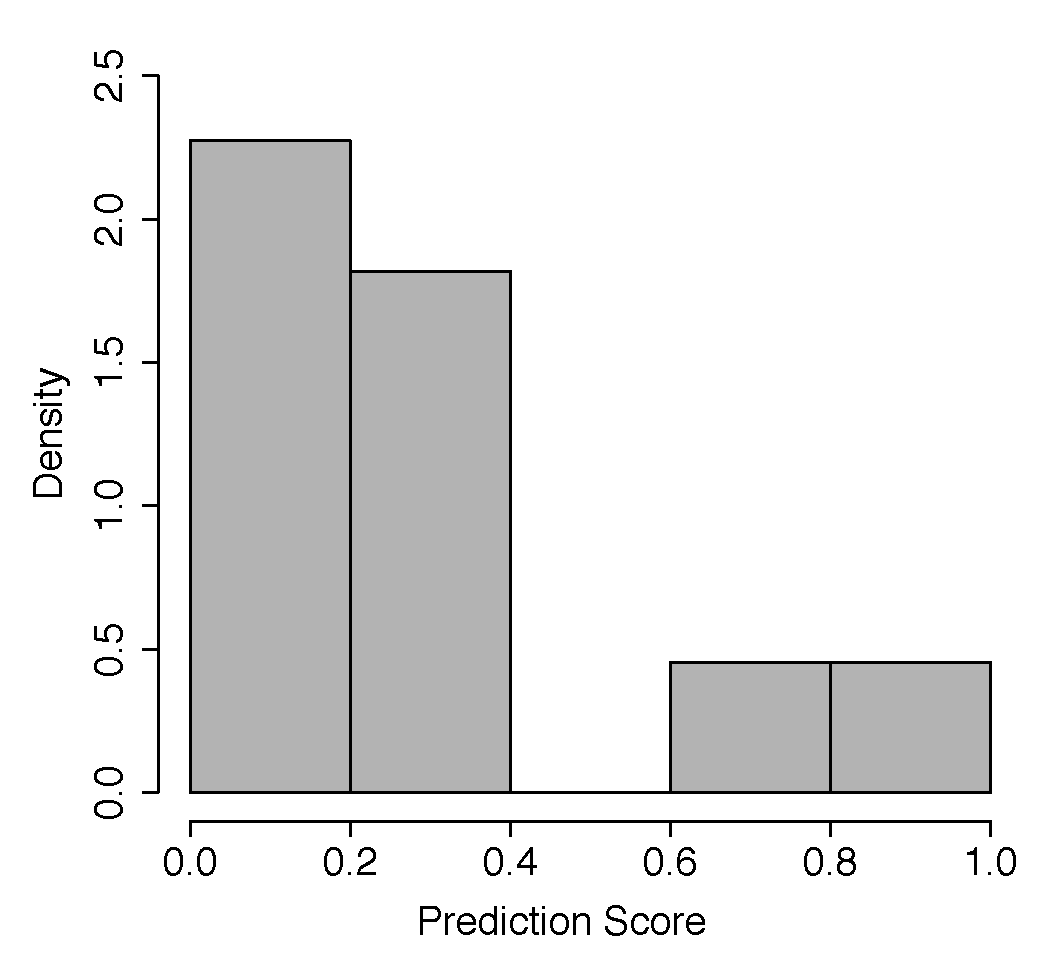
\includegraphics[width=0.4\textwidth]{images/Eval-ScoreDistributionsSpam.pdf}}
			\subfigure[ham]{\label{fig:scoreExampleHistosNonSpam}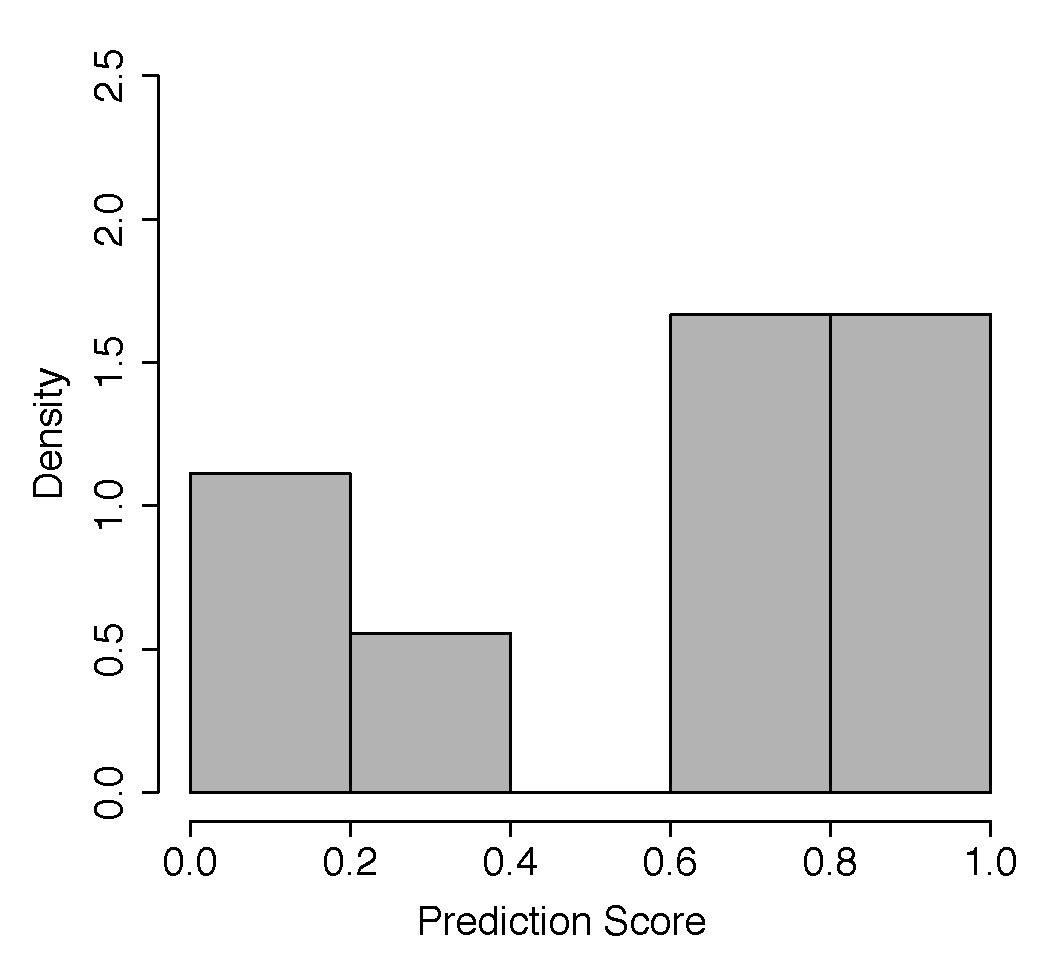
\includegraphics[width=0.4\textwidth]{images/Eval-ScoreDistributionsNonSpam.pdf}}
       \caption{Prediction score distributions for the (a) \featL{spam} and (b) \featL{ham} target levels based on the data in Table \ourRef{tab:samplePredictionExampleExtended}.}
       \label{fig:scoreExampleHistos}
       \end{centering}
\end{figure}
\end{frame} 

\subsection{Receiver Operating Characteristic Curves}

\begin{frame}
	\begin{itemize}
		\item The \alert{receiver operating characteristic index} (\alert{ROC index}), which is based on the \alert{receiver operating characteristic curve} (\alert{ROC curve}), is a widely used performance measure that is calculated using prediction scores. 
		\item TPR and TNR are intrinsically tied to the threshold used to convert prediction scores into target levels. 
		\item This threshold can be changed, however, which leads to different predictions and a different confusion matrix. 
	\end{itemize}
\end{frame}

 \begin{frame} 
\begin{table}
\caption{Confusion matrices for the set of predictions shown in Table \ourRef{tab:samplePredictionExampleExtended} using (a) a prediction score threshold of \alert{$0.75$} and (b) a prediction score threshold of \alert{$0.25$}.}
\label{tab:confusionMatrixExampleModified}
\centering
\begin{footnotesize}
\subtable[Threshold: 0.75]{\label{tab:confusionMatrixExampleModified0_75}\begin{tabular}{c >{\bfseries}r @{\hspace{0.7em}} | c @{\hspace{0.4em}} c @{\hspace{0.7em}}}
    & &  \multicolumn{2}{c}{\bfseries Prediction} \\
  & & \bfseries \featL{spam} & \bfseries \featL{ham} \\
  \hline
  \multirow{2}{*}{\parbox{1.1cm}{\bfseries\raggedleft Target}}  & \featL{spam} & $4$	&	$4$ \\
  & \featL{ham} & $2$	&	$10$ 
\end{tabular}}
\subtable[Threshold: 0.25]{\label{tab:confusionMatrixExampleModified0_25}\begin{tabular}{c >{\bfseries}r @{\hspace{0.7em}} | c @{\hspace{0.4em}} c @{\hspace{0.7em}}}
    & &  \multicolumn{2}{c}{\bfseries Prediction} \\
  & & \bfseries \featL{spam} & \bfseries \featL{ham} \\
  \hline
  \multirow{2}{*}{\parbox{1.1cm}{\bfseries\raggedleft Target}}  & \featL{spam} & $7$	&	$2$ \\
  & \featL{ham} & $4$	&	$7$ 
\end{tabular}}
\end{footnotesize}
\end{table}
\end{frame} 



 \begin{frame} [plain]
\begin{table}[!tb]
%\caption{A sample test set with prediction scores and resulting predictions based on different threshold values.}
\label{tab:samplePredictionExampleChaginingThresh}
\centering
\begin{scriptsize}
\begin{tabular}{  c  c  c  c  c  c  c  c }
\hline
~	 &  &  & Pred. & Pred. & Pred. & Pred. & Pred.	 \\
\featN{ID}	 & Target & Score & (0.10) & (0.25) & (0.50) & (0.75) & (0.90)	 \\
\hline
7	&	ham	&	0.001	&	ham	&	ham	&	ham	&	ham	&	ham	\\
11	&	ham	&	0.003	&	ham	&	ham	&	ham	&	ham	&	ham	\\
15	&	ham	&	0.059	&	ham	&	ham	&	ham	&	ham	&	ham	\\
13	&	ham	&	0.064	&	ham	&	ham	&	ham	&	ham	&	ham	\\
19	&	ham	&	0.094	&	ham	&	ham	&	ham	&	ham	&	ham	\\
12	&	spam	&	0.160	&	spam	&	ham	&	ham	&	ham	&	ham	\\
2	&	spam	&	0.184	&	spam	&	ham	&	ham	&	ham	&	ham	\\
3	&	ham	&	0.226	&	spam	&	ham	&	ham	&	ham	&	ham	\\
16	&	ham	&	0.246	&	spam	&	ham	&	ham	&	ham	&	ham	\\
1	&	spam	&	0.293	&	spam	&	spam	&	ham	&	ham	&	ham	\\
5	&	ham	&	0.302	&	spam	&	spam	&	ham	&	ham	&	ham	\\
14	&	ham	&	0.348	&	spam	&	spam	&	ham	&	ham	&	ham	\\
17	&	ham	&	0.657	&	spam	&	spam	&	spam	&	ham	&	ham	\\
8	&	spam	&	0.676	&	spam	&	spam	&	spam	&	ham	&	ham	\\
6	&	spam	&	0.719	&	spam	&	spam	&	spam	&	ham	&	ham	\\
10	&	spam	&	0.781	&	spam	&	spam	&	spam	&	spam	&	ham	\\
18	&	spam	&	0.833	&	spam	&	spam	&	spam	&	spam	&	ham	\\
20	&	ham	&	0.877	&	spam	&	spam	&	spam	&	spam	&	ham	\\
9	&	spam	&	0.960	&	spam	&	spam	&	spam	&	spam	&	spam	\\
4	&	spam	&	0.963	&	spam	&	spam	&	spam	&	spam	&	spam	\\									
\hline 
\multicolumn{3}{r}{\textbf{Misclassification Rate}}	&	0.300	&	0.300	&	0.250	&	0.300	&	0.350	\\
\multicolumn{3}{r}{\textbf{True Positive Rate (TPR)}}	&	1.000	&	0.778	&	0.667	&	0.444	&	0.222	\\
\multicolumn{3}{r}{\textbf{True Negative rate (TNR)}}	&	0.455	&	0.636	&	0.818	&	0.909	&	1.000	\\
\multicolumn{3}{r}{\textbf{False Positive Rate (FPR)}}	&	0.545	&	0.364	&	0.182	&	0.091	&	0.000	\\
\multicolumn{3}{r}{\textbf{False Negative Rate (FNR)}}	&	0.000	&	0.222	&	0.333	&	0.556	&	0.778	\\
\hline 
\end{tabular}
\end{scriptsize}
\end{table}
\end{frame} 

\begin{frame}
	\begin{itemize}
		\item Note: as the threshold increases TPR decreases and TNR increases (and vice versa).
		\item Capturing this tradeoff is the basis of the ROC curve.
	\end{itemize}
\end{frame}

 \begin{frame} 
\begin{figure}[!bth]
       \begin{centering}
		\subfigure[]{\label{fig:TPRandTNRvsThresh}\includegraphics[width=0.48\textwidth]{images/Eval-TPRandTNRvsThresh.pdf}}
		\subfigure[]{\label{fig:rocPoints}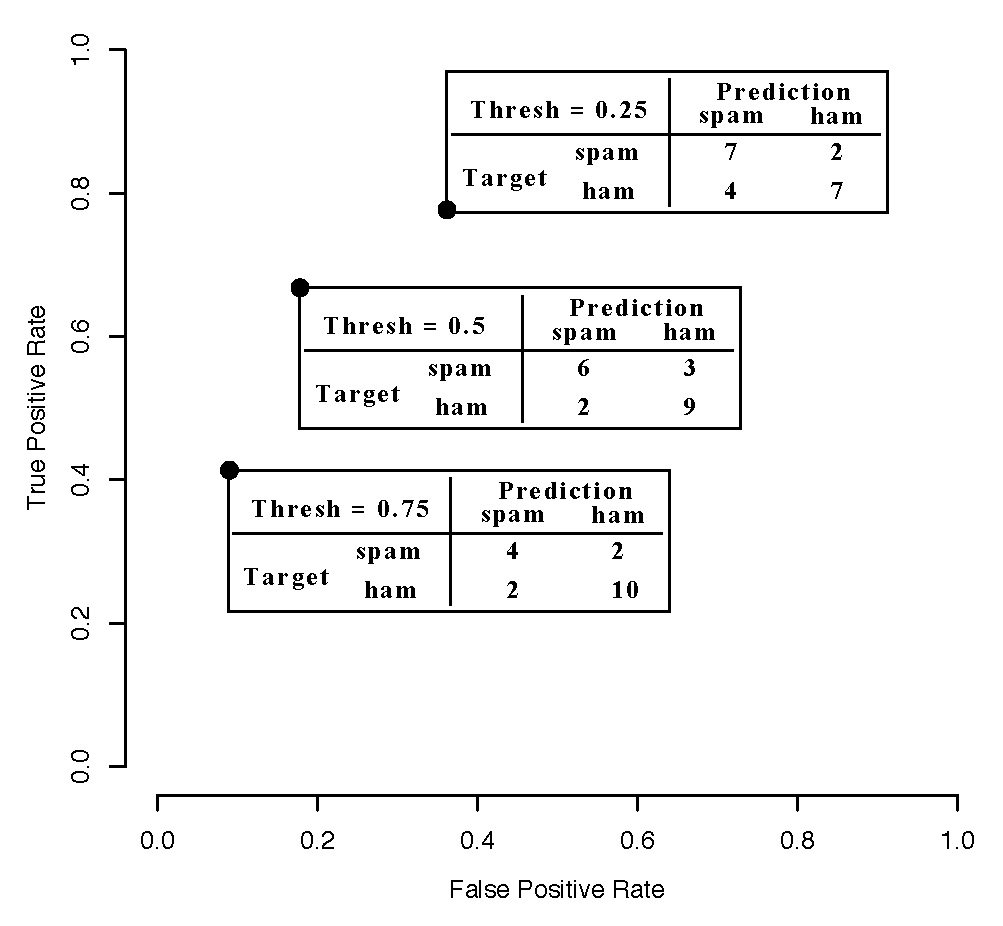
\includegraphics[width=0.48\textwidth]{images/Eval-ROCPointsMod3.pdf}}
       \caption{(a) The changing values of TPR and TNR for the test data shown in Table \ourRef{tab:samplePredictionExampleChaginingThresh} as the threshold is altered; (b) points in ROC space for thresholds of $0.25$, $0.5$, and $0.75$.}
       \end{centering}
       \label{fig:rocPanels1}
\end{figure}
\end{frame} 

 \begin{frame} 
\begin{figure}[!bth]
       \begin{centering}
		\subfigure[]{\label{fig:rocCurveExample}\includegraphics[width=0.48\textwidth]{images/Eval-ROCCurve.pdf}}
		\subfigure[]{\label{fig:rocCurveMultiple}\includegraphics[width=0.48\textwidth]{images/Eval-ROCCurve-Multiple.pdf}}
       \caption{(a) A complete ROC curve for the email classification example; (b) a selection of ROC curves for different models trained on the same prediction task.}
       \end{centering}
       \label{fig:rocPanels2}
\end{figure}
\end{frame} 

 \begin{frame} 
  \begin{itemize}
	\item We can also calculate a single performance measure from an ROC curve
	\item The \alert{ROC Index} measures the area underneath an ROC curve.
\end{itemize}
\begin{alignat}{2}
&\text{ROC index} = \notag\\ 
&\sum_{i=2}^{|\mathbf{T}|} \frac{\left( FPR(\mathbf{T}[i]) - FPR(\mathbf{T}[i-1]) \right) \times  \left( TPR(\mathbf{T}[i]) + TPR(\mathbf{T}[i-1])\right)}{2} \label{eqn:rocIndex}
\end{alignat}
\end{frame} 

 \begin{frame} 
  \begin{itemize}
	\item The \keyword{Gini coefficient} is a linear rescaling of the ROC index
\end{itemize}
\begin{alignat}{2}
\text{Gini coefficient} & =  (2 \times \text{ROC index}) - 1 \label{eqn:giniIndex}
\end{alignat}
\end{frame} 

\subsection{Kolmogorov-Smirnov Statistic}

 \begin{frame} 
 \begin{itemize}
 	\item  The \keyword{Kolmogorov-Smirnov statistic} (\alert{K-S statistic}) is another performance measure that captures the separation between the distribution of prediction scores for the different target levels in a classification problem. 
\end{itemize}
\end{frame}

\begin{frame}
	\begin{itemize}
	\item To calculate the K-S statistic, we first determine the cumulative probability distributions of the prediction scores for the positive and negative target levels:
	\begin{scriptsize}
\begin{alignat}{2}
CP(positive, ps) =  \frac{\text{num positive test instances with score $\leq ps$}}{\text{num positive test instances}} \\
CP(negative, ps) =  \frac{\text{num  negative test instances with score $\leq ps$}}{\text{num negative test instances}}
\end{alignat}
\end{scriptsize}
\end{itemize}
\end{frame}

 \begin{frame} 
\begin{figure}[htb]
       \begin{centering}
			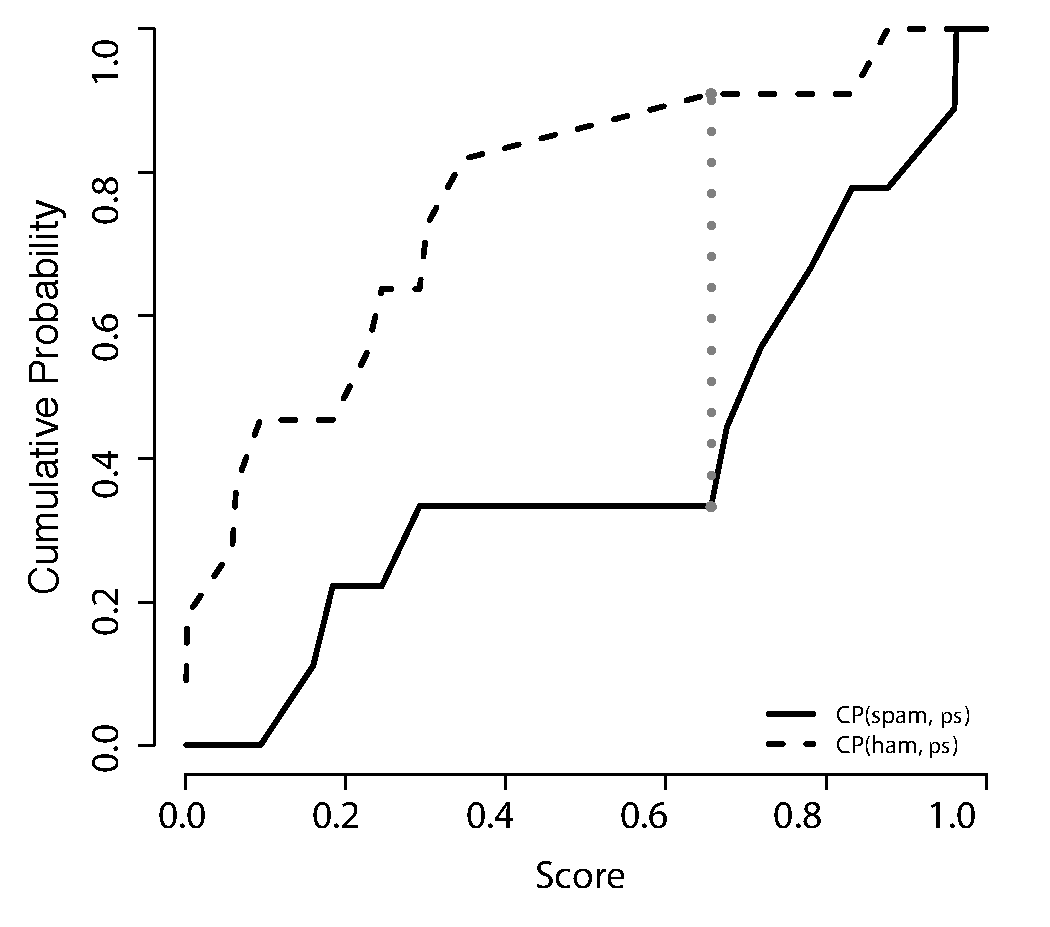
\includegraphics[width=0.48\textwidth]{images/Eval-KS-Curves.pdf}
       \caption{The K-S chart for the email classification predictions shown in Table \ourRef{tab:samplePredictionExampleExtended}.}
       \label{fig:ksCurveExample}
       \end{centering}
\end{figure}
\end{frame} 

 \begin{frame} 
  \begin{itemize}
 	\item The K-S statistic is calculated by determining the maximum difference between the cumulative probability distributions for the positive and negative target levels. 
\end{itemize}

\begin{alignat}{2}
\text{K-S} & =  \underset{ps}{max}\left(CP(positive, ps) - CP(negative, ps)\right) 
\end{alignat}
\end{frame} 

\begin{frame} [plain]
\begin{table}[!htb]
%\caption{Tabulating the workings required to generate a K-S statistic.}
\label{tab:ksStatExampleWorkings}
\centering
\begin{scriptsize}
\begin{tabular}{  c  c  c  c  c  c  c }
\hline
~	&	~		& Positive	&	Negative	&	Positive 	&	Negative	 &	~	\\
~	&	~	 & 	(\featL{spam})	&	(\featL{ham})	&	(\featL{spam}) 	&	(\featL{ham})	 &	~	\\
~	&	Prediction	& Cumulative	&	Cumulative	&	Cumulative 	&	Cumulative	 &	~	\\
\featN{ID}	&	Score	 &	Count	&	Count	&	Probability 	& Probability	 &	Distance	\\
\hline
7	&	0.001 & 0	&	1	&	0.000	&	0.091	&	0.091	\\
11	&	0.003 & 	0	&	2	&	0.000	&	0.182	&	0.182	\\
15	&	0.059 & 	0	&	3	&	0.000	&	0.273	&	0.273	\\
13	&	0.064 & 	0	&	4	&	0.000	&	0.364	&	0.364	\\
19	&	0.094 & 	0	&	5	&	0.000	&	0.455	&	0.455	\\
12	&	0.160 & 	1	&	5	&	0.111	&	0.455	&	0.343	\\
2	&	0.184 & 	2	&	5	&	0.222	&	0.455	&	0.232	\\
3	&	0.226 & 	2	&	6	&	0.222	&	0.545	&	0.323	\\
16	&	0.246 & 	2	&	7	&	0.222	&	0.636	&	0.414	\\
1	&	0.293 & 	3	&	7	&	0.333	&	0.636	&	0.303	\\
5	&	0.302 & 	3	&	8	&	0.333	&	0.727	&	0.394	\\
14	&	0.348 & 	3	&	9	&	0.333	&	0.818	&	0.485	\\
\textbf{17}	&	\textbf{0.657} & 	\textbf{3}	&	\textbf{10}	&	\textbf{0.333}	&	\textbf{0.909}	&	\textbf{0.576*}	\\
8	&	0.676 & 	4	&	10	&	0.444	&	0.909	&	0.465	\\
6	&	0.719 & 	5	&	10	&	0.556	&	0.909	&	0.354	\\
10	&	0.781 & 	6	&	10	&	0.667	&	0.909	&	0.242	\\
18	&	0.833 & 	7	&	10	&	0.778	&	0.909	&	0.131	\\
20	&	0.877 & 	7	&	11	&	0.778	&	1.000	&	0.222	\\
9	&	0.960 & 	8	&	11	&	0.889	&	1.000	&	0.111	\\
4	&	0.963 & 	9	&	11	&	1.000	&	1.000	&	0.000	\\
\hline
\end{tabular}
\end{scriptsize}
\end{table}
\end{frame} 

\subsection{Measuring Gain and Lift}

 \begin{frame} [plain]
\begin{figure}[!thb]
       \begin{centering}
 			\subfigure[Model 1]{\label{fig:bigKSExamplesNonSpamDistStrip1}\includegraphics[width=0.24\textwidth]{images/Strip.pdf}}
			\subfigure[Model 2]{\label{fig:bigKSExamplesNonSpamDistStrip2}\includegraphics[width=0.24\textwidth]{images/Strip.pdf}}
			\subfigure[Model 3]{\label{fig:bigKSExamplesNonSpamDistStrip3}\includegraphics[width=0.24\textwidth]{images/Strip.pdf}}
			\subfigure[Model 4]{\label{fig:bigKSExamplesNonSpamDistStrip4}\includegraphics[width=0.24\textwidth]{images/Strip.pdf}}	
 			\subfigure{\label{fig:bigKSExamplesNonSpamDist1}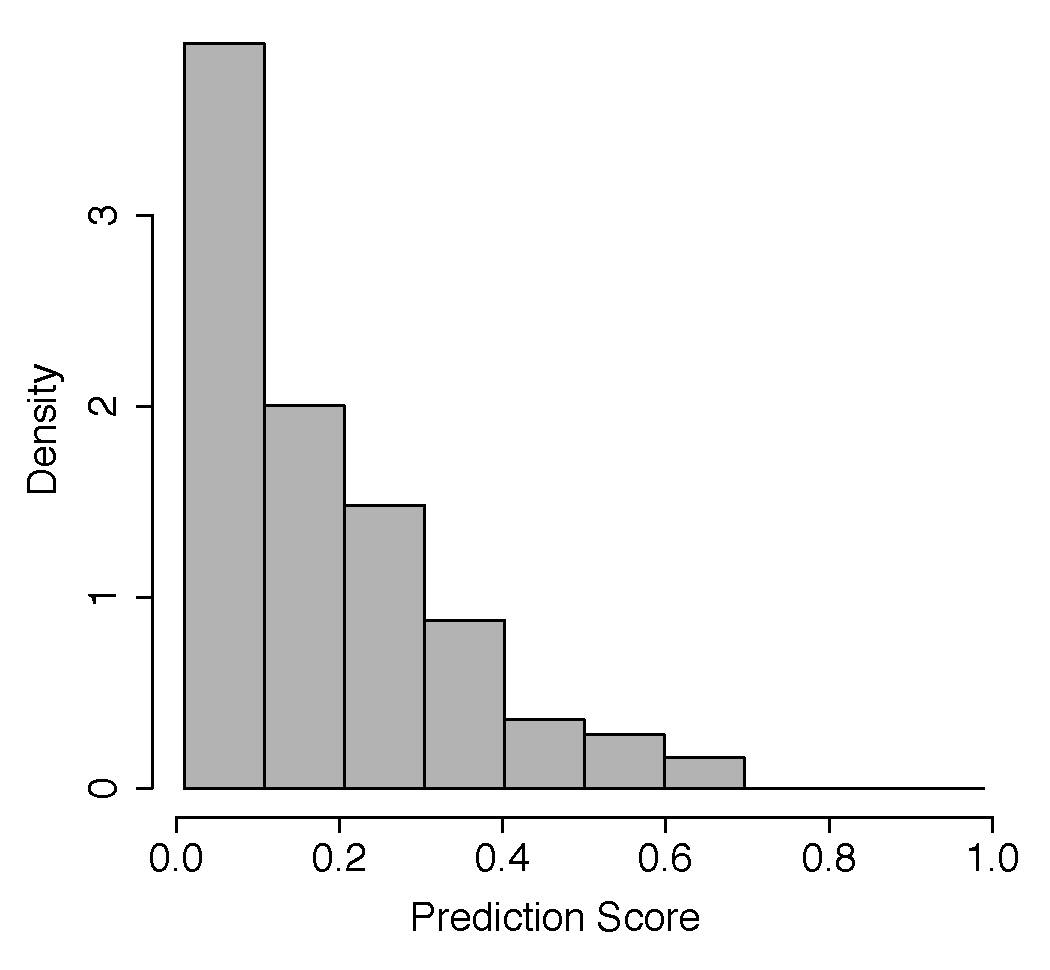
\includegraphics[width=0.24\textwidth]{images/Eval-ScoreDistributionsNonSpam1.pdf}}
			\subfigure{\label{fig:bigKSExamplesNonSpamDist2}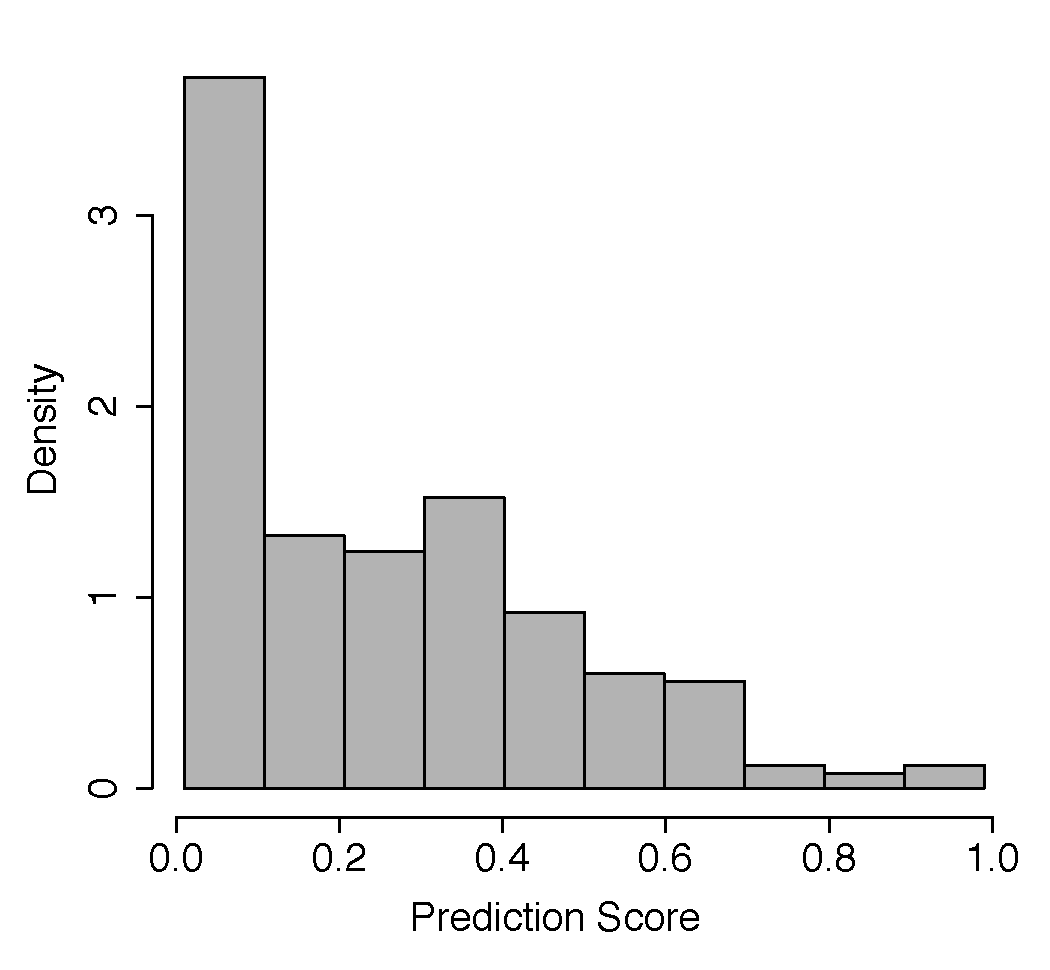
\includegraphics[width=0.24\textwidth]{images/Eval-ScoreDistributionsNonSpam2.pdf}}
			\subfigure{\label{fig:bigKSExamplesNonSpamDist3}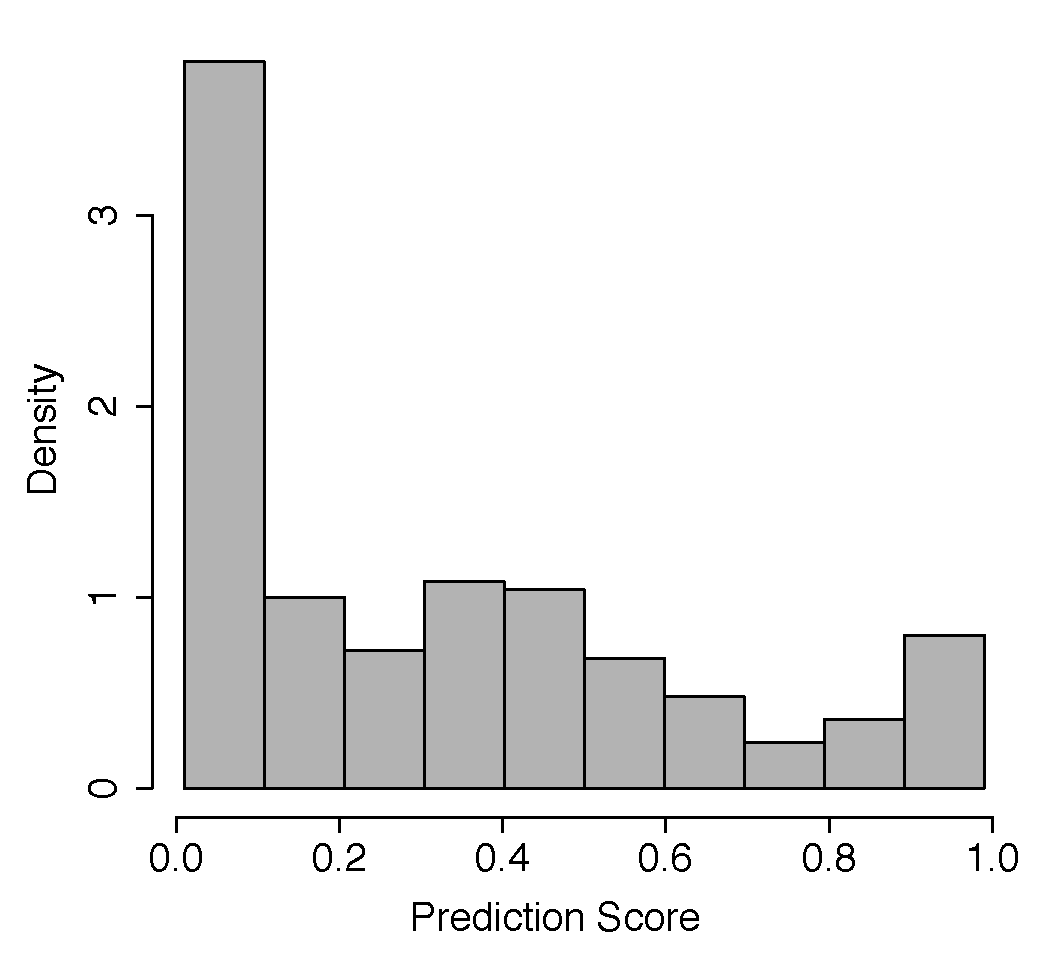
\includegraphics[width=0.24\textwidth]{images/Eval-ScoreDistributionsNonSpam3.pdf}}
			\subfigure{\label{fig:bigKSExamplesNonSpamDist4}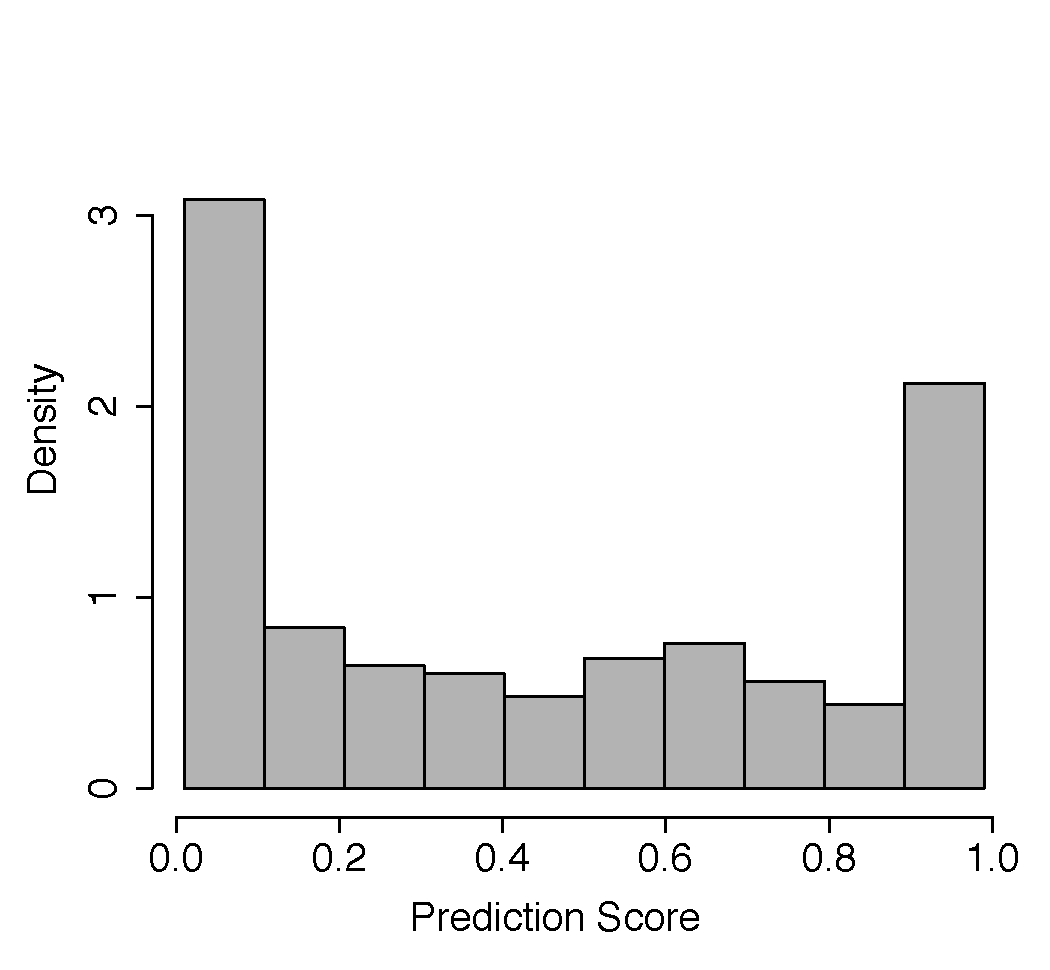
\includegraphics[width=0.24\textwidth]{images/Eval-ScoreDistributionsNonSpam4.pdf}}			
       			\subfigure{\label{fig:bigKSExamplesSpamDist1}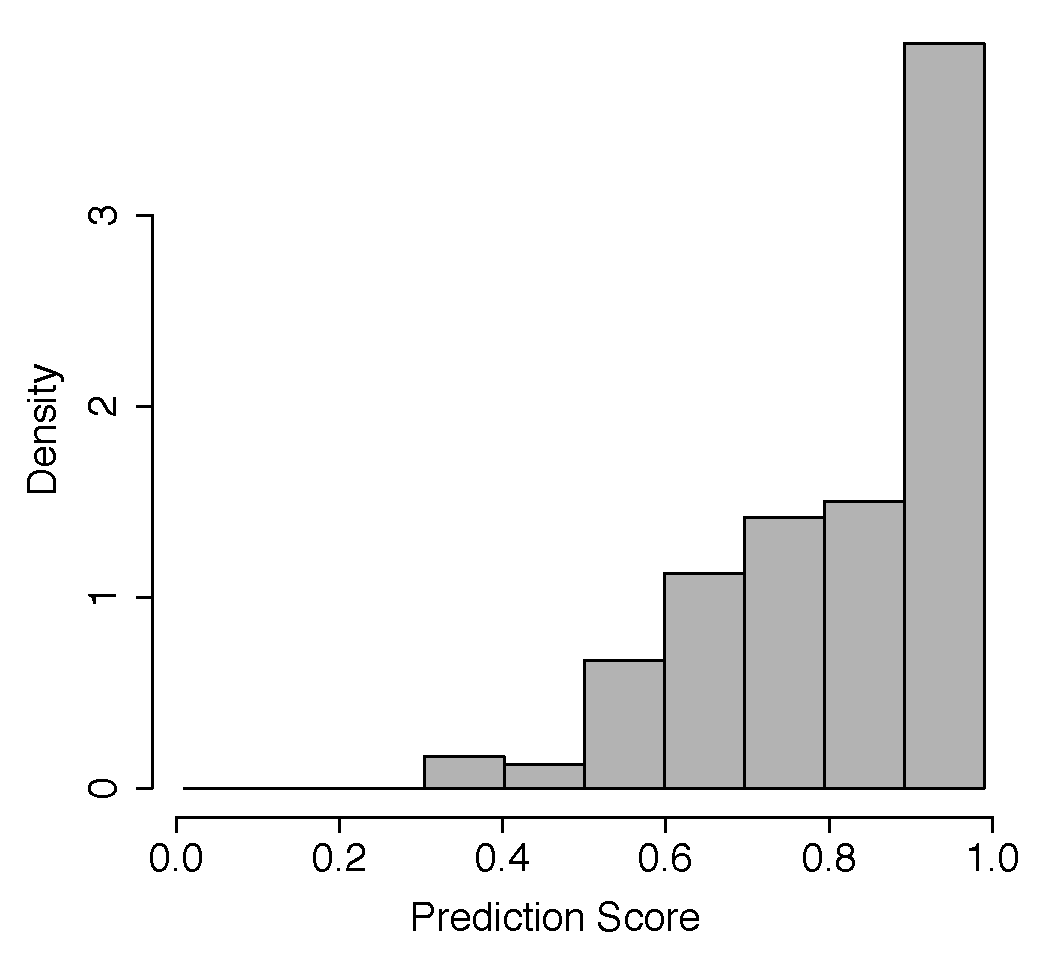
\includegraphics[width=0.24\textwidth]{images/Eval-ScoreDistributionsSpam1.pdf}}
			\subfigure{\label{fig:bigKSExamplesSpamDist2}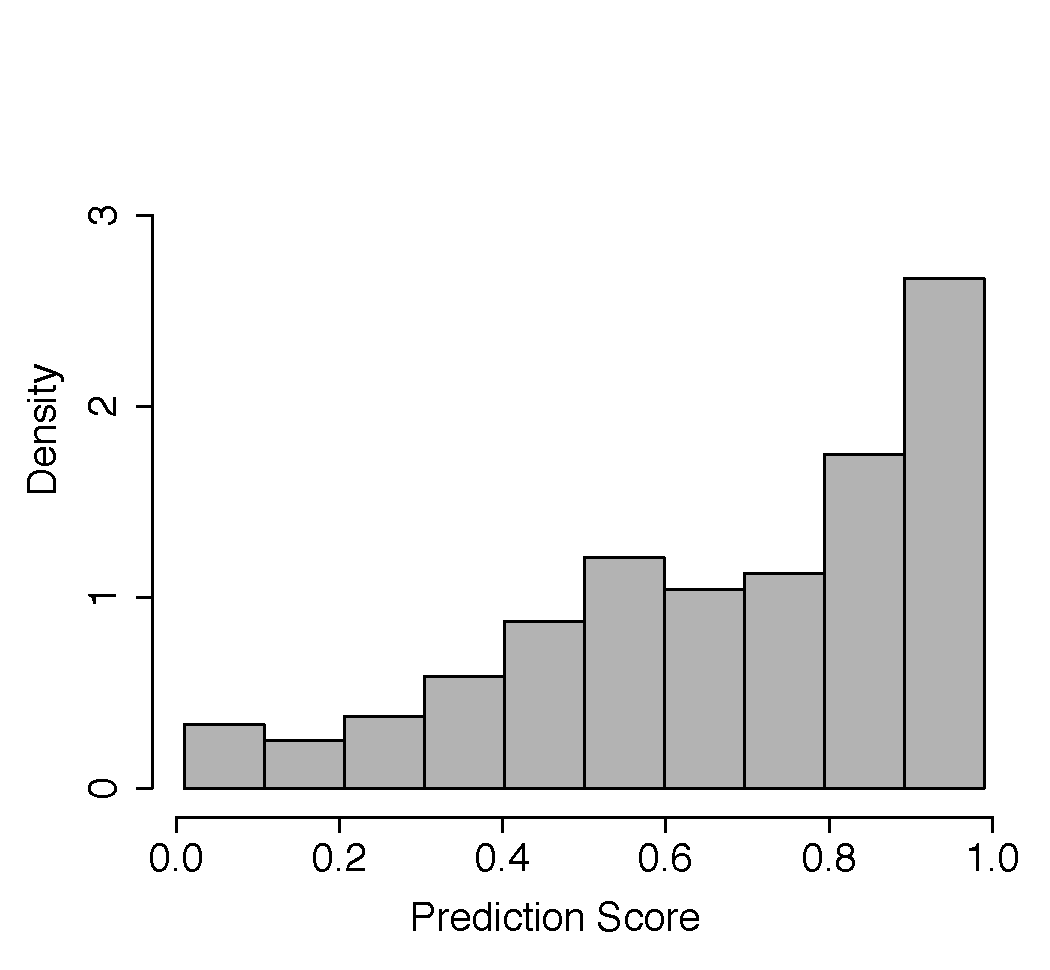
\includegraphics[width=0.24\textwidth]{images/Eval-ScoreDistributionsSpam2.pdf}}
			\subfigure{\label{fig:bigKSExamplesSpamDist3}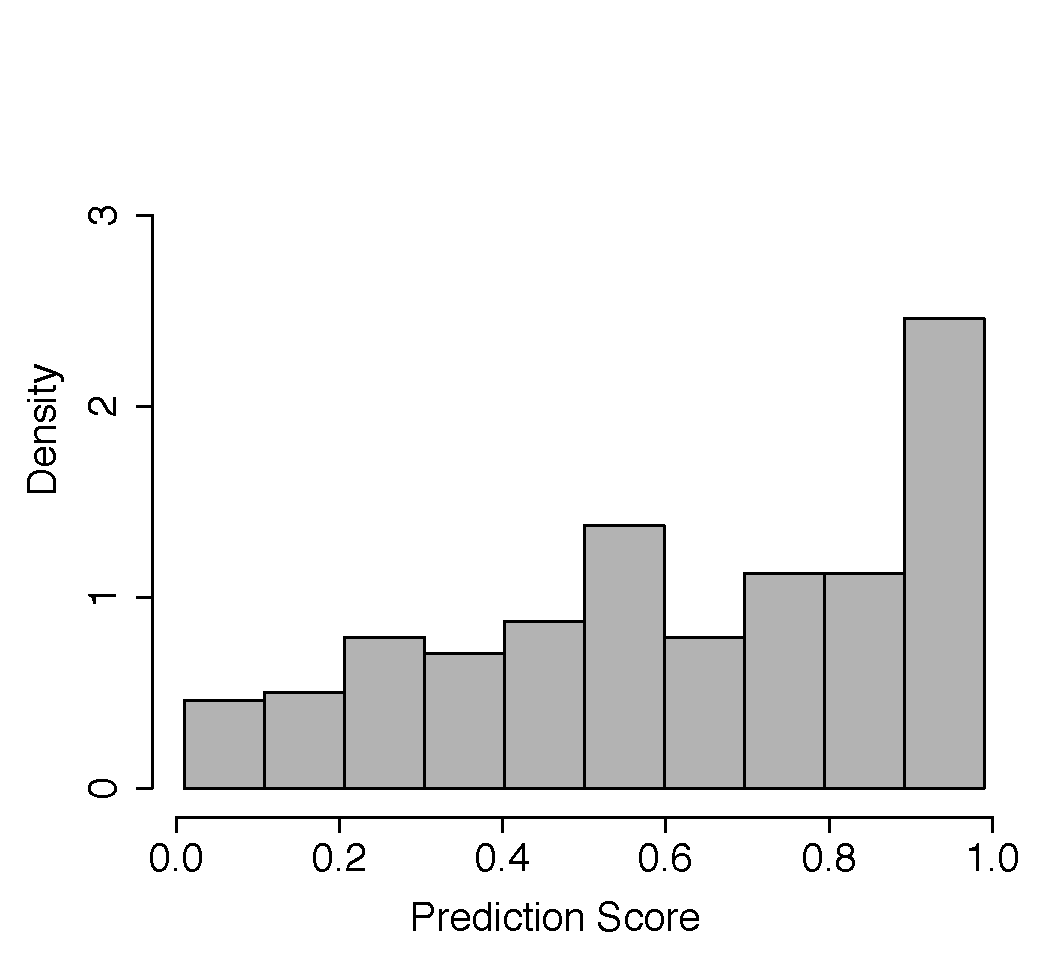
\includegraphics[width=0.24\textwidth]{images/Eval-ScoreDistributionsSpam3.pdf}}
			\subfigure{\label{fig:bigKSExamplesSpamDist4}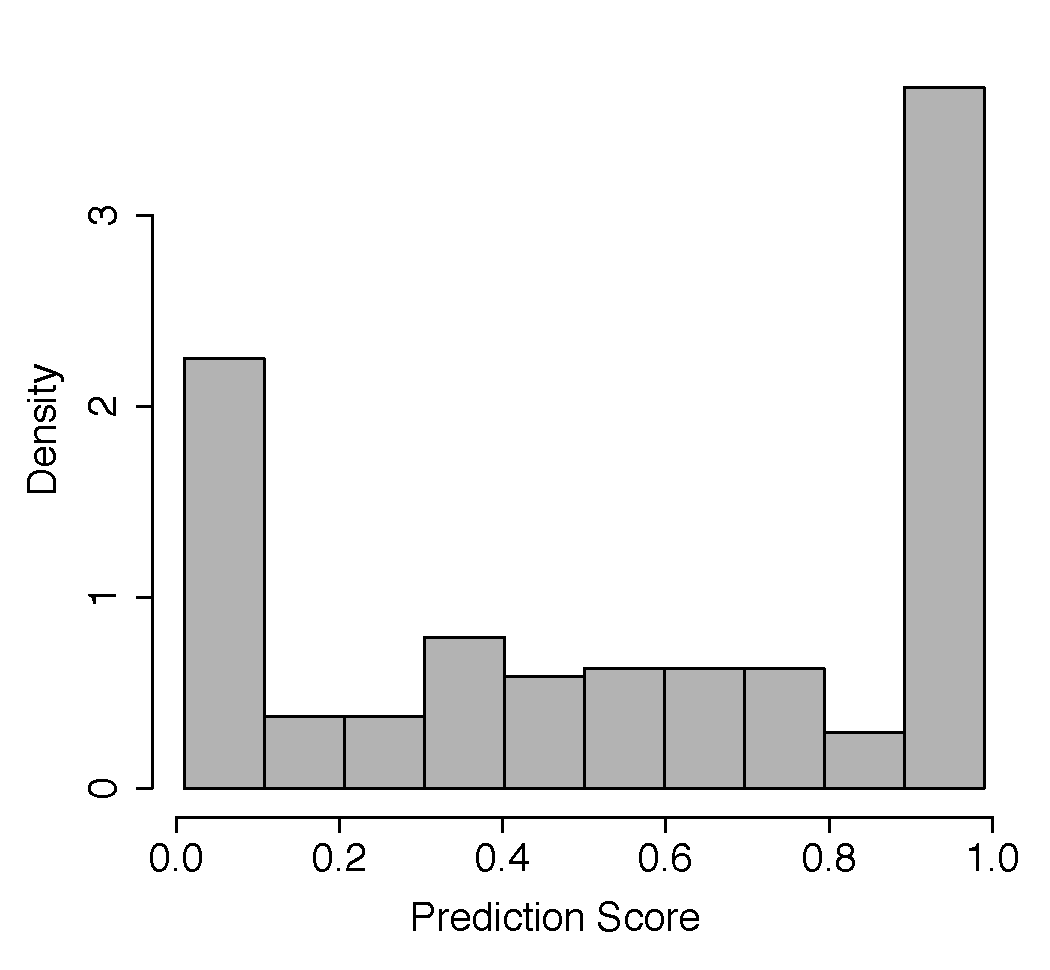
\includegraphics[width=0.24\textwidth]{images/Eval-ScoreDistributionsSpam4.pdf}}			
			\subfigure{\label{fig:bigKSExamplesKS1}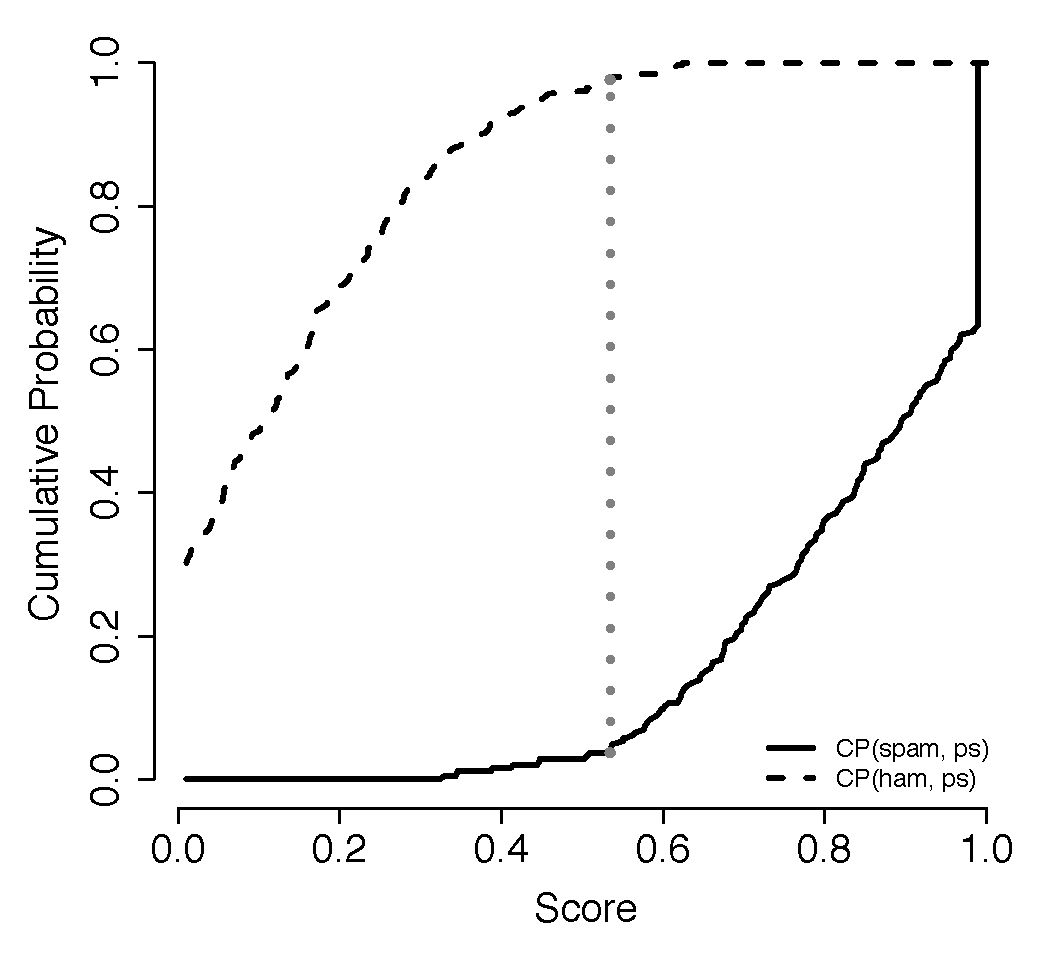
\includegraphics[width=0.24\textwidth]{images/Eval-KS-Curves1.pdf}}
			\subfigure{\label{fig:bigKSExamplesKS2}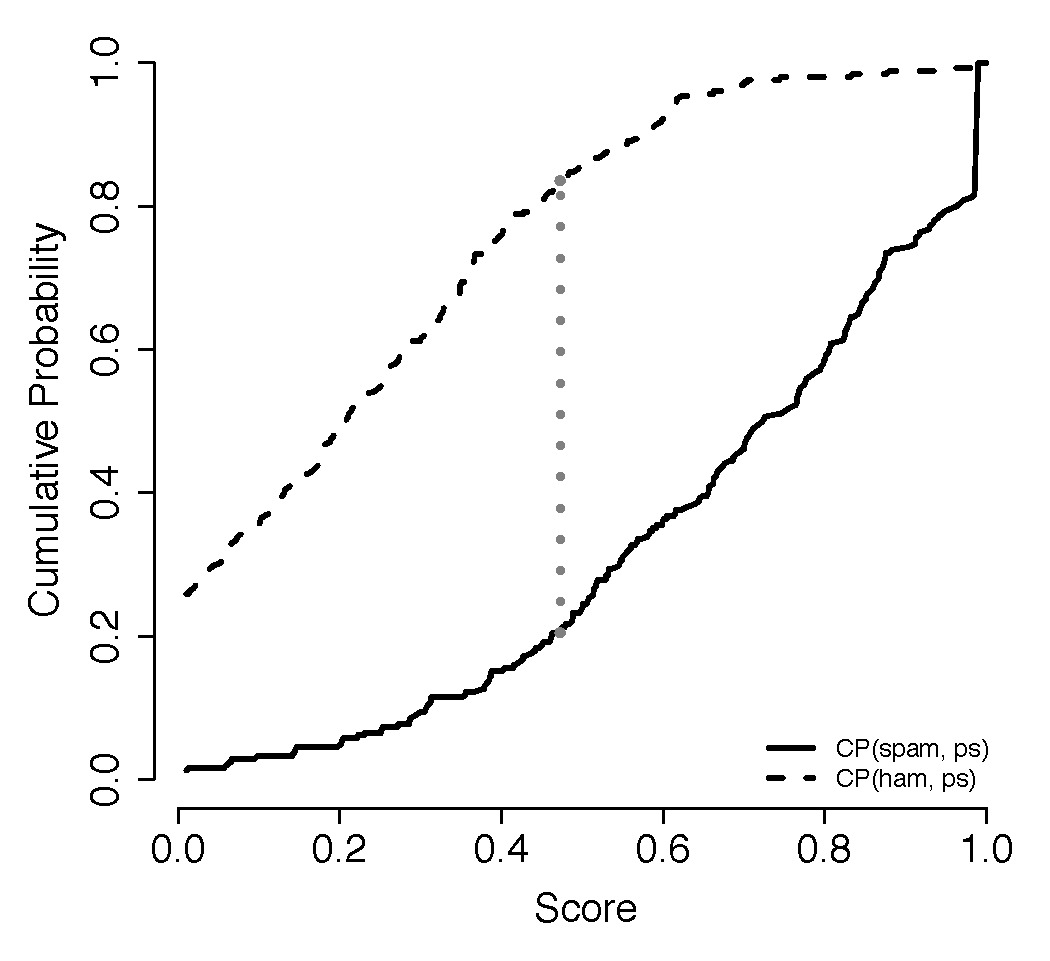
\includegraphics[width=0.24\textwidth]{images/Eval-KS-Curves2.pdf}}
			\subfigure{\label{fig:bigKSExamplesKS3}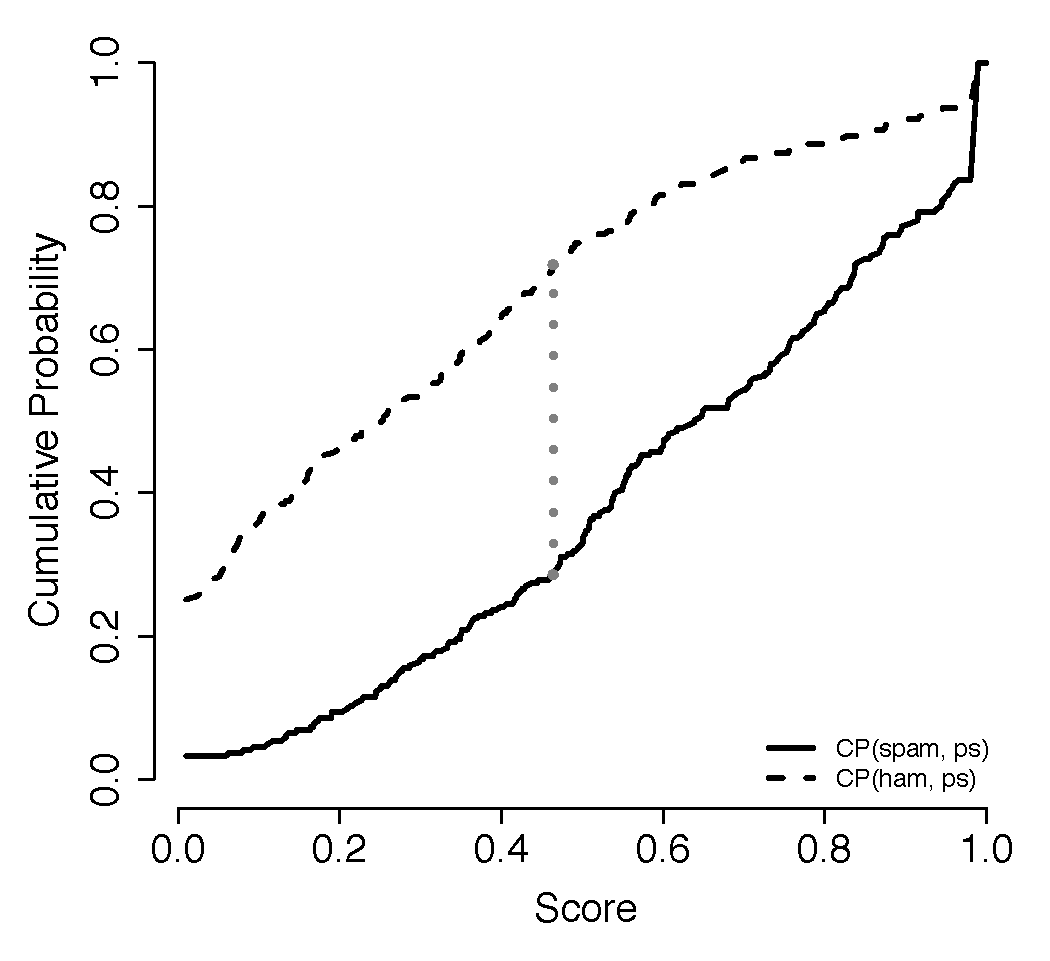
\includegraphics[width=0.24\textwidth]{images/Eval-KS-Curves3.pdf}}
			\subfigure{\label{fig:bigKSExamplesKS4}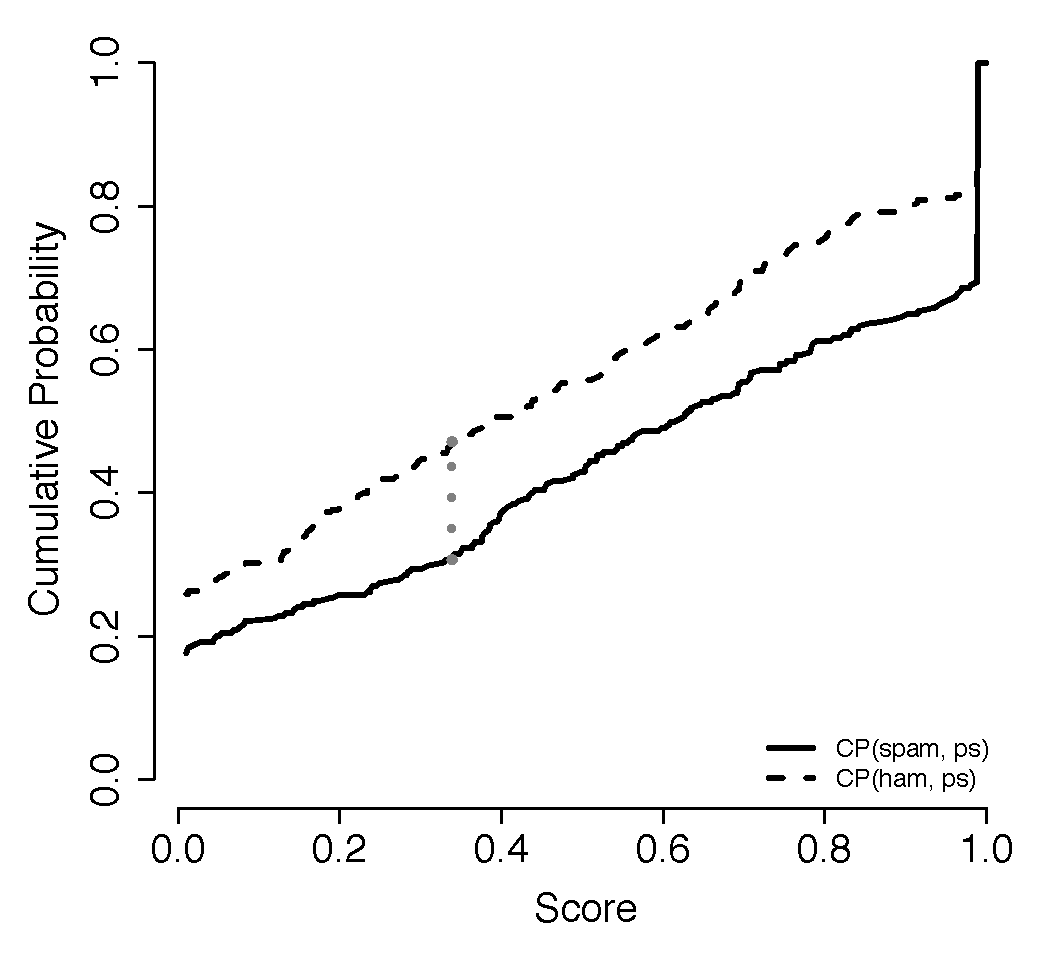
\includegraphics[width=0.24\textwidth]{images/Eval-KS-Curves4.pdf}}			
       \caption{A series of charts for different model performance on the same large email classification test set used to generate the ROC curves in Figure \ourRef{fig:rocCurveMultiple}. Each column from top to bottom: a histogram of the \featL{ham} scores predicted by the model, a histogram of the \featL{spam} scores predicted by the model, and the K-S chart.}
       \label{fig:bigKSExamples}
       \end{centering}
\end{figure}
\end{frame} 

 \begin{frame} [plain]
\begin{table}[!tb]
\caption{The test set with model predictions and scores from Table \ourRef{tab:samplePredictionExampleExtended} extended to include deciles.}
\label{tab:samplePredictionExampleExtendedWithDeciles}
\centering
\begin{scriptsize}
\begin{tabular}{ c c  c  c  c  c }
\hline
Decile & \featN{ID}	 & Target & Prediction & Score & Outcome\\
\hline 
\multirow{2}{*}{ $1^{st}$} & 9	&	spam	&	spam	&	0.960	&	TP	\\
 & 4	&	spam	&	spam	&	0.963	&	TP	\\
 \hdashline
 \multirow{2}{*}{ $2^{nd}$} & 18	&	spam	&	spam	&	0.833	&	TP	\\
 & 20	&	ham	&	spam	&	0.877	&	FP	\\
\hdashline
\multirow{2}{*}{ $3^{rd}$} & 6	&	spam	&	spam	&	0.719	&	TP	\\
 & 10	&	spam	&	spam	&	0.781	&	TP	\\
 \hdashline
\multirow{2}{*}{ $4^{th}$} & 17	&	ham	&	spam	&	0.657	&	FP	\\
 & 8	&	spam	&	spam	&	0.676	&	TP	\\
 \hdashline
\multirow{2}{*}{ $5^{th}$} & 5	&	ham	&	ham	&	0.302	&	TN	\\
 & 14	&	ham	&	ham	&	0.348	&	TN	\\
 \hdashline
\multirow{2}{*}{ $6^{th}$} & 16	&	ham	&	ham	&	0.246	&	TN	\\
 & 1	&	spam	&	ham	&	0.293	&	FN	\\
 \hdashline
\multirow{2}{*}{ $7^{th}$} & 2	&	spam	&	ham	&	0.184	&	FN	\\
 & 3	&	ham	&	ham	&	0.226	&	TN	\\
 \hdashline
\multirow{2}{*}{ $8^{th}$} & 19	&	ham	&	ham	&	0.094	&	TN	\\
 & 12	&	spam	&	ham	&	0.160	&	FN	\\
 \hdashline
\multirow{2}{*}{ $9^{th}$} & 15	&	ham	&	ham	&	0.059	&	TN	\\
 & 13	&	ham	&	ham	&	0.064	&	TN	\\
 \hdashline
\multirow{2}{*}{ $10^{th}$} & 7	&	ham	&	ham	&	0.001	&	TN	\\
 & 11	&	ham	&	ham	&	0.003	&	TN	\\
\hline 
\end{tabular}
\end{scriptsize}
\end{table}
\end{frame} 

 \begin{frame} 
 \begin{footnotesize}
\begin{alignat}{2}
\text{Gain}(dec) =
 \frac{\text{num positive test instances in decile $dec$}}{\text{num positive test instances}}
\label{eqn:gain}
\end{alignat}
\end{footnotesize}
\end{frame} 

 \begin{frame} 
\begin{table}[!tb]
\caption{Tabulating the workings required to calculate \indexkeyword{gain}, \indexkeyword{cumulative gain}, \indexkeyword{lift}, and \indexkeyword{cumulative lift} for the data given in Table \ourRef{tab:samplePredictionExampleExtended}.}
\label{tab:gainLiftExampleWorkings}
\centering
\begin{footnotesize}
\begin{tabular}{ c  c  c  c  c  c  c  c  c }
\hline
Decile	& \pbox[b]{20cm}{Positive \\ (\featL{spam}) \\ Count}	&	\pbox[b]{20cm}{Negative \\ (\featL{ham}) \\ Count}	&	Gain	&	\pbox[b]{20cm}{Cum. \\ Gain} & Lift	&	\pbox[b]{20cm}{Cum. \\ Lift}	\\
\hline
$1^{st}$	&	2	&	0	&	0.222	&	0.222	& 2.222	&	2.222	\\
$2^{nd}$	&	1	&	1	&	0.111	&	0.333	&	1.111	&	1.667	\\
$3^{rd}$	&	2	&	0	&	0.222	&	0.556	&	2.222	&	1.852	\\
$4^{th}$		&	1	&	1	&	0.111	&	0.667	&	1.111	&	1.667	\\
$5^{th}$		&	0	&	2	&	0.000	&	0.667	&	0.000	&	1.333	\\
$6^{th}$		&	1	&	1	&	0.111	&	0.778	&	1.111	&	1.296	\\
$7^{th}$		&	1	&	1	&	0.111	&	0.889	&	1.111	&	1.270	\\
$8^{th}$		&	1	&	1	&	0.111	&	1.000	&	1.111	&	1.250	\\
$9^{th}$		&	0	&	2	&	0.000	&	1.000	&	0.000	&	1.111	\\
$10^{th}$		&	0	&	2	&	0.000		&	1.000	&	0.000	&	1.000	\\
\hline 
\end{tabular}
\end{footnotesize}
\end{table}
\end{frame} 


 \begin{frame} 
 \begin{footnotesize}
\begin{alignat}{2}
\text{Cumulative gain}(dec) =  \frac{\text{num positive test instances in all deciles up to $dec$}}{\text{num positive test instances}}
\end{alignat}
\end{footnotesize}
\end{frame} 


 \begin{frame} 
\begin{figure}[htb]
       \begin{centering}
			\subfigure[]{\label{fig:gainsExample}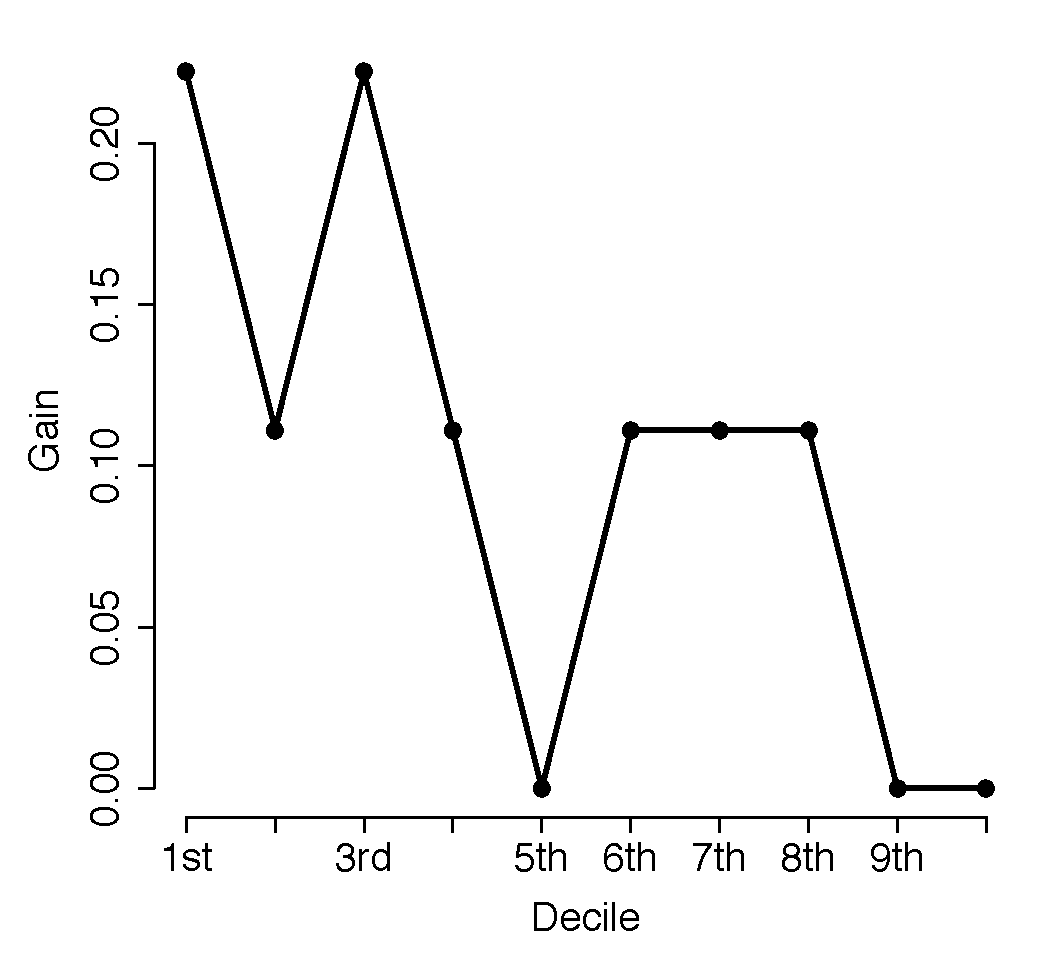
\includegraphics[width=0.4\textwidth]{images/Eval-GainsChart.pdf}}
			\subfigure[]{\label{fig:cumGainsExample}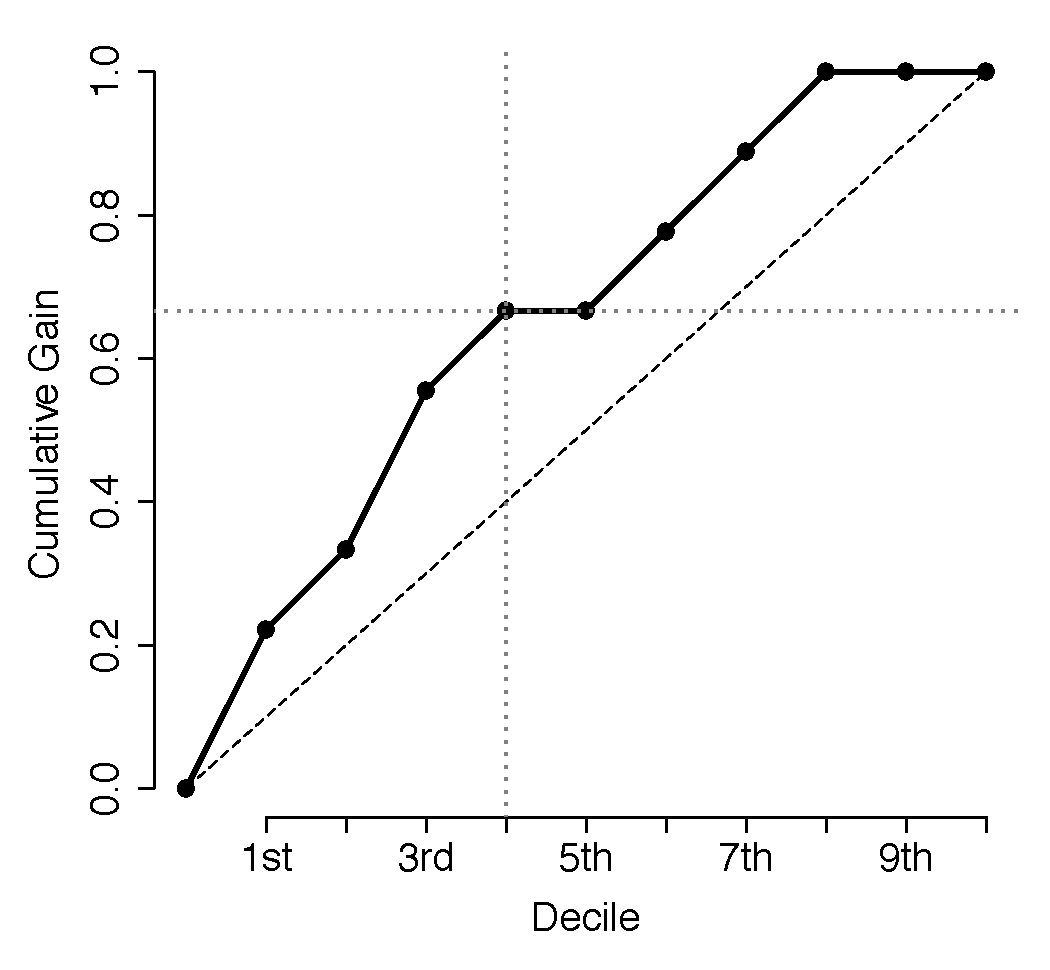
\includegraphics[width=0.4\textwidth]{images/Eval-CumulativeGainsChart.pdf}}
       \caption{The (a) \indexkeyword{gain} and (b)  \indexkeyword{cumulative gain} at each decile for the email predictions given in Table \ourRef{tab:samplePredictionExampleExtended}.}
       \label{fig:gainExamples}
       \end{centering}
\end{figure}
\end{frame} 


 \begin{frame} 
\begin{footnotesize}
\begin{alignat}{2}
\text{Lift}(dec) =  \frac{\text{\% of positive test instances in decile $dec$}}{\text{\% of positive test instances}}
\end{alignat}
\end{footnotesize}
\end{frame} 


 \begin{frame} 
\begin{figure}[htb]
       \begin{centering}
			\subfigure[]{\label{fig:liftExample}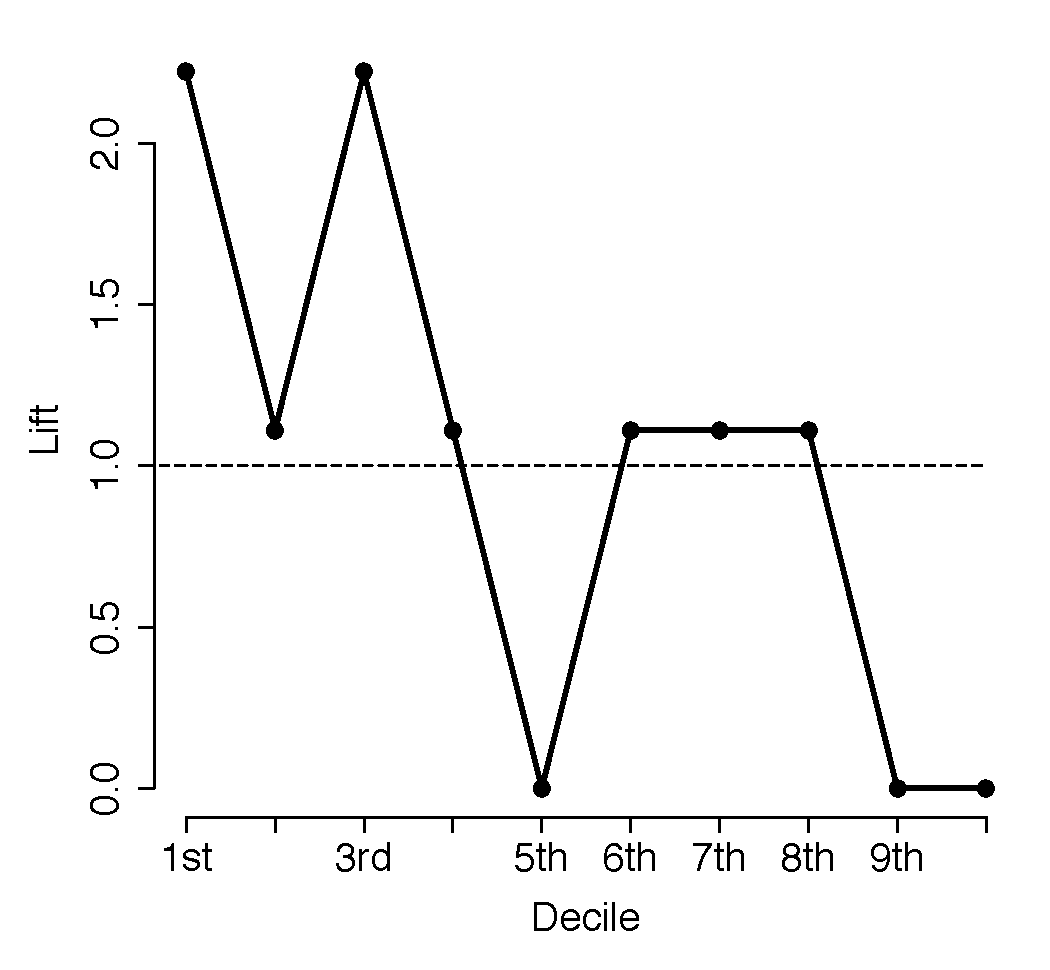
\includegraphics[width=0.4\textwidth]{images/Eval-LiftChart.pdf}}
			\subfigure[]{\label{fig:cumulativeLiftExample}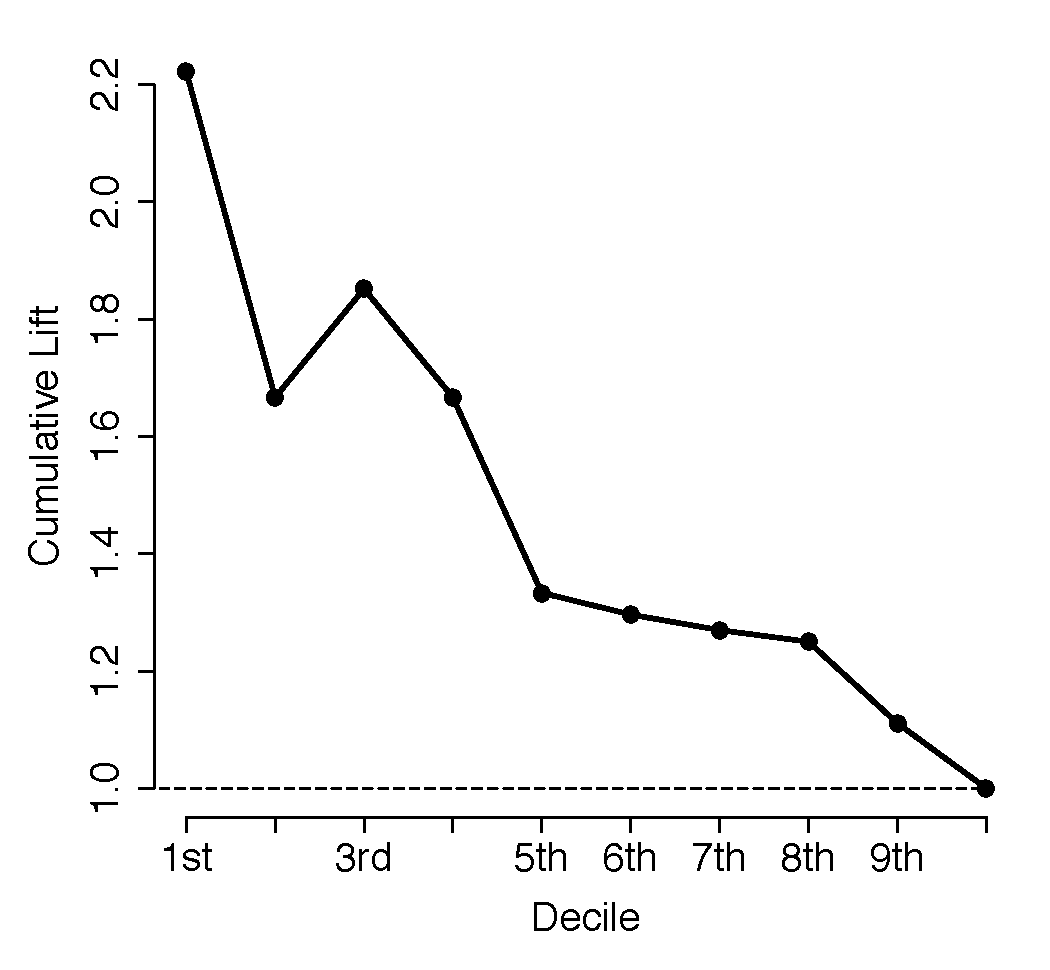
\includegraphics[width=0.4\textwidth]{images/Eval-CumulativeLiftChart.pdf}}	
       \caption{The (a) \indexkeyword{lift} and (b) \indexkeyword{cumulative lift} at each decile for the email predictions given in Table \ourRef{tab:samplePredictionExampleExtended}.}
       \label{fig:liftExamples}
       \end{centering}
\end{figure}
\end{frame} 


 \begin{frame} 
\begin{alignat}{2}
\text{Cumulative lift}(dec) =  \frac{\text{\% of positive instances in all deciles up to $dec$}}{\text{\% of positive test instances}}
\end{alignat}
\end{frame} 


 \begin{frame} [plain]
\begin{figure}[htb]
       \begin{centering}
        			\subfigure[Model 1]{\label{fig:bigLiftGainExamplesDistStrip1}\includegraphics[width=0.24\textwidth]{images/Strip.pdf}}
			\subfigure[Model 2]{\label{fig:bigLiftGainExamplesDistStrip2}\includegraphics[width=0.24\textwidth]{images/Strip.pdf}}
			\subfigure[Model 3]{\label{fig:bigLiftGainExamplesDistStrip3}\includegraphics[width=0.24\textwidth]{images/Strip.pdf}}
			\subfigure[Model 4]{\label{fig:bigLiftGainExamplesDistStrip4}\includegraphics[width=0.24\textwidth]{images/Strip.pdf}}		
						
       		\subfigure{\label{fig:bigLiftGainExamplesCumGains1}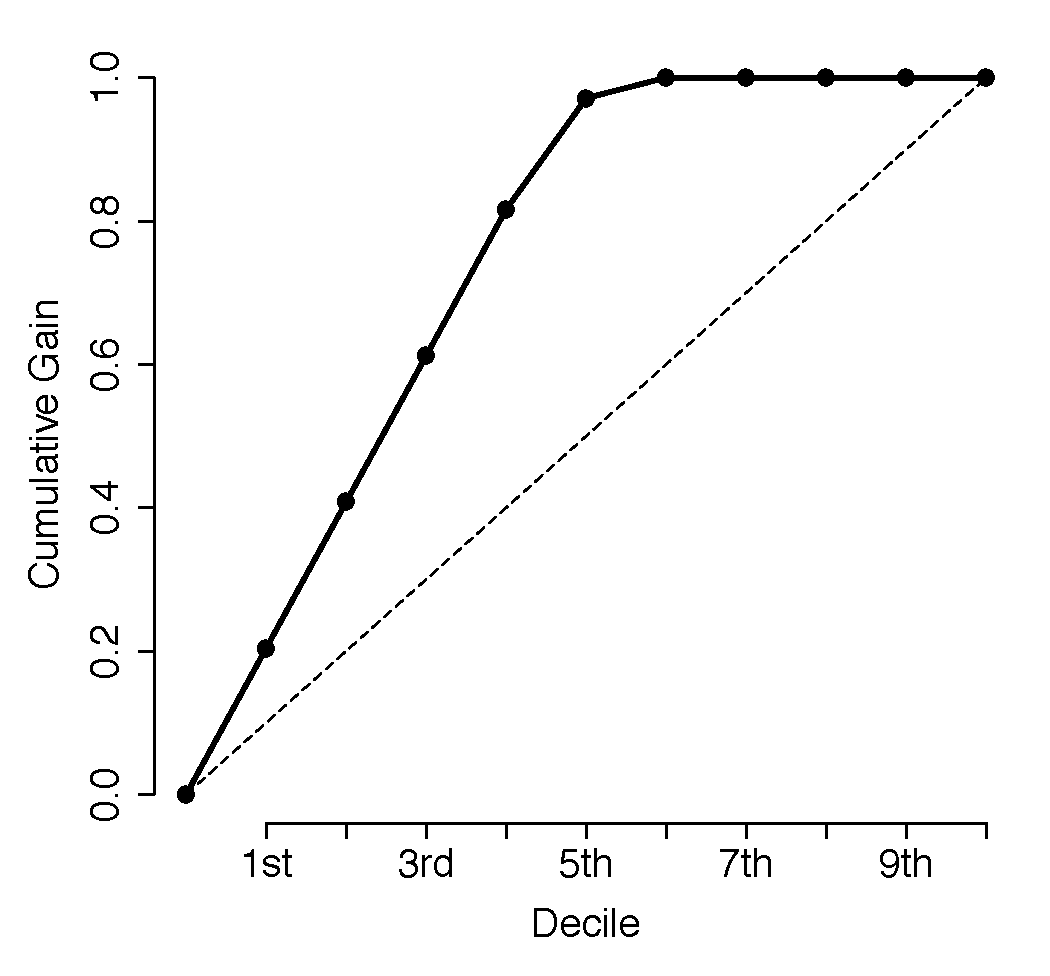
\includegraphics[width=0.24\textwidth]{images/Eval-CumulativeGainsChart1.pdf}}
    			\subfigure{\label{fig:bigLiftGainExamplesCumGains2}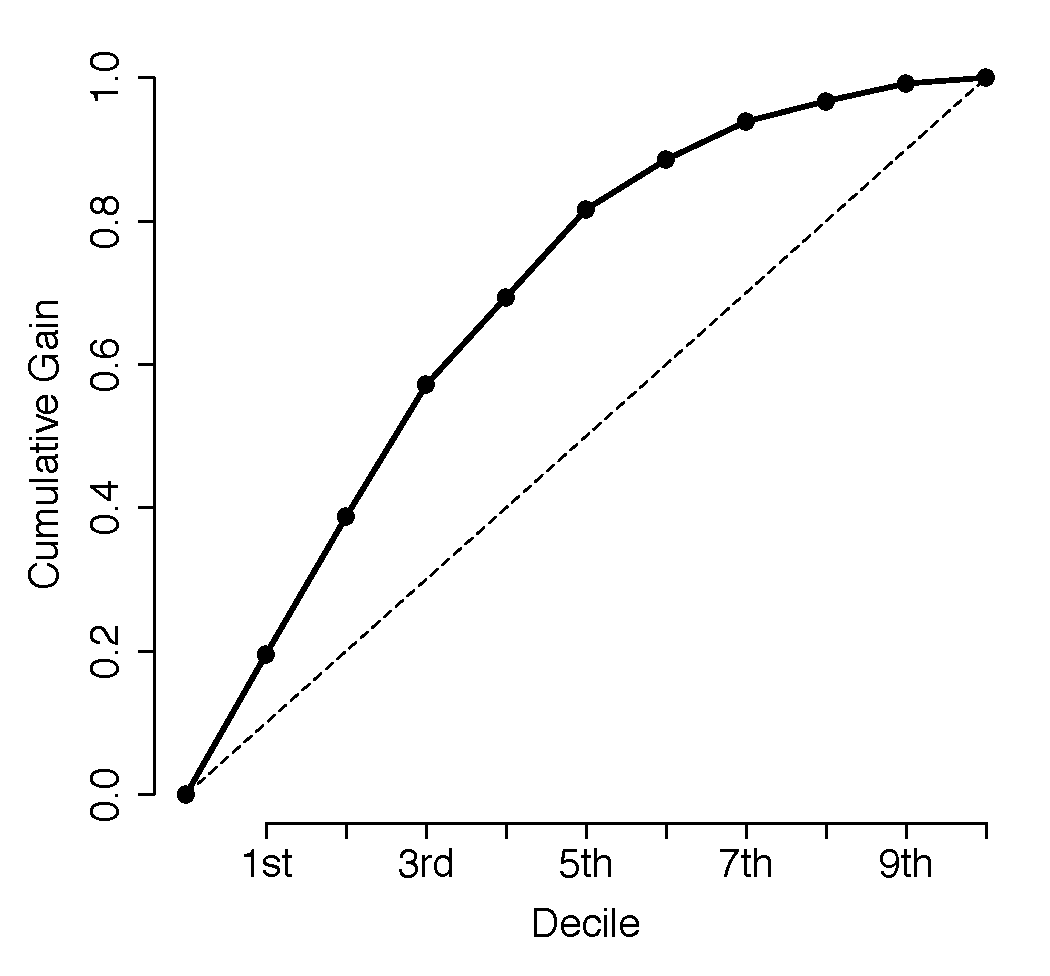
\includegraphics[width=0.24\textwidth]{images/Eval-CumulativeGainsChart2.pdf}}
			\subfigure{\label{fig:bigLiftGainExamplesCumGains3}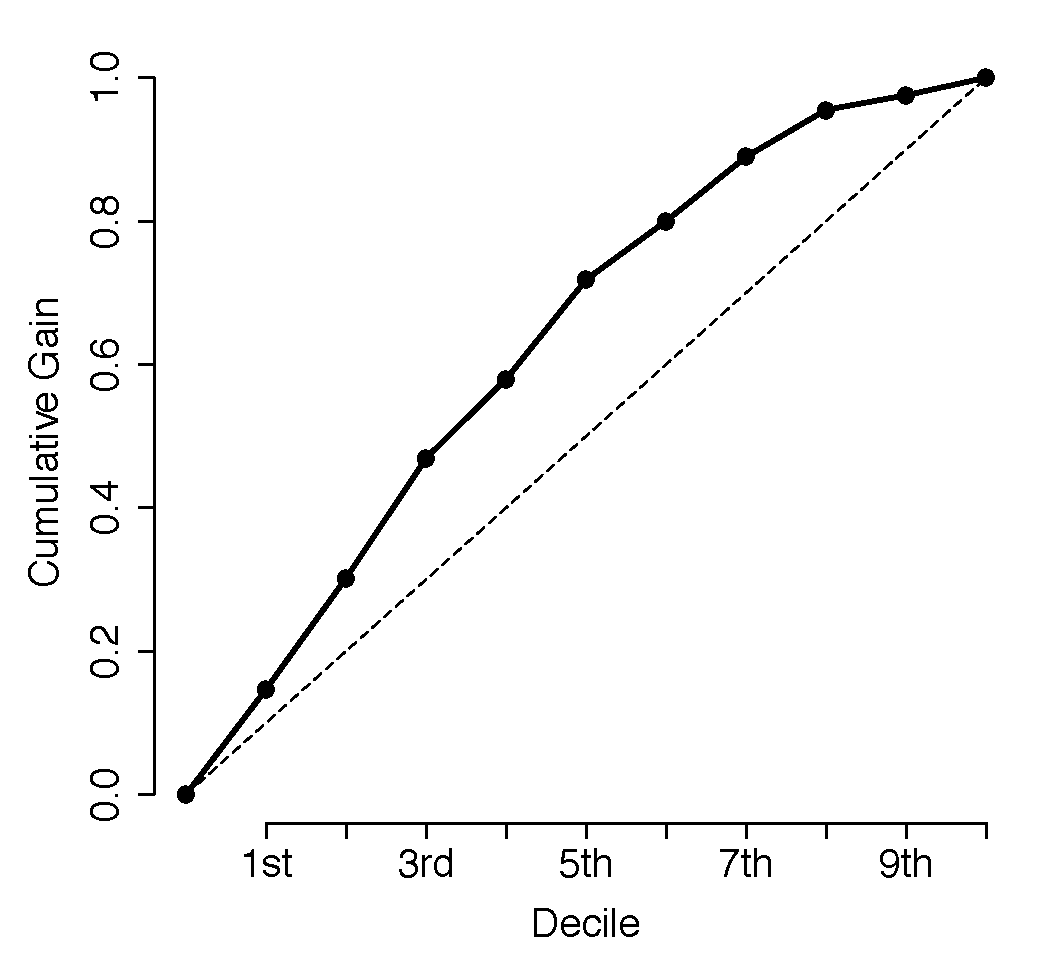
\includegraphics[width=0.24\textwidth]{images/Eval-CumulativeGainsChart3.pdf}}
			\subfigure{\label{fig:bigLiftGainExamplesCumGains4}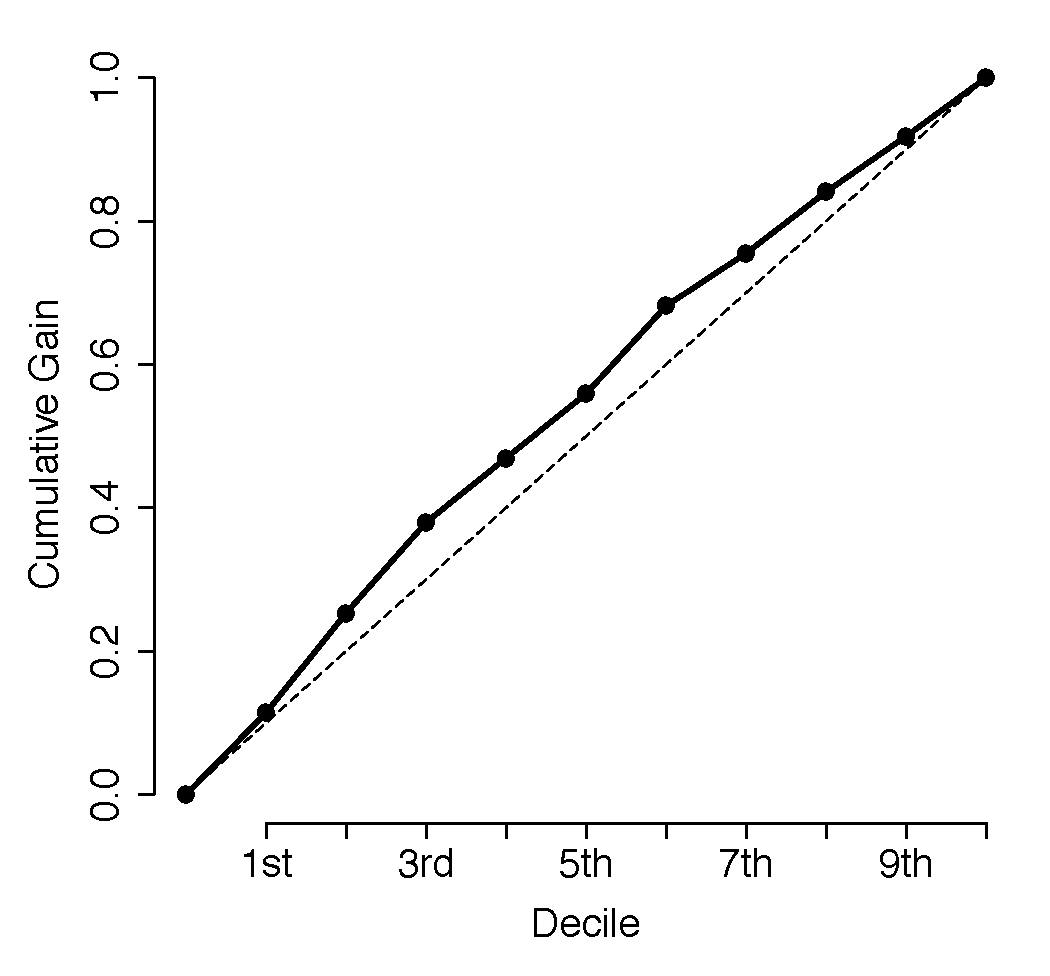
\includegraphics[width=0.24\textwidth]{images/Eval-CumulativeGainsChart4.pdf}}
						
			\subfigure{\label{fig:bigLiftGainExamplesLift1}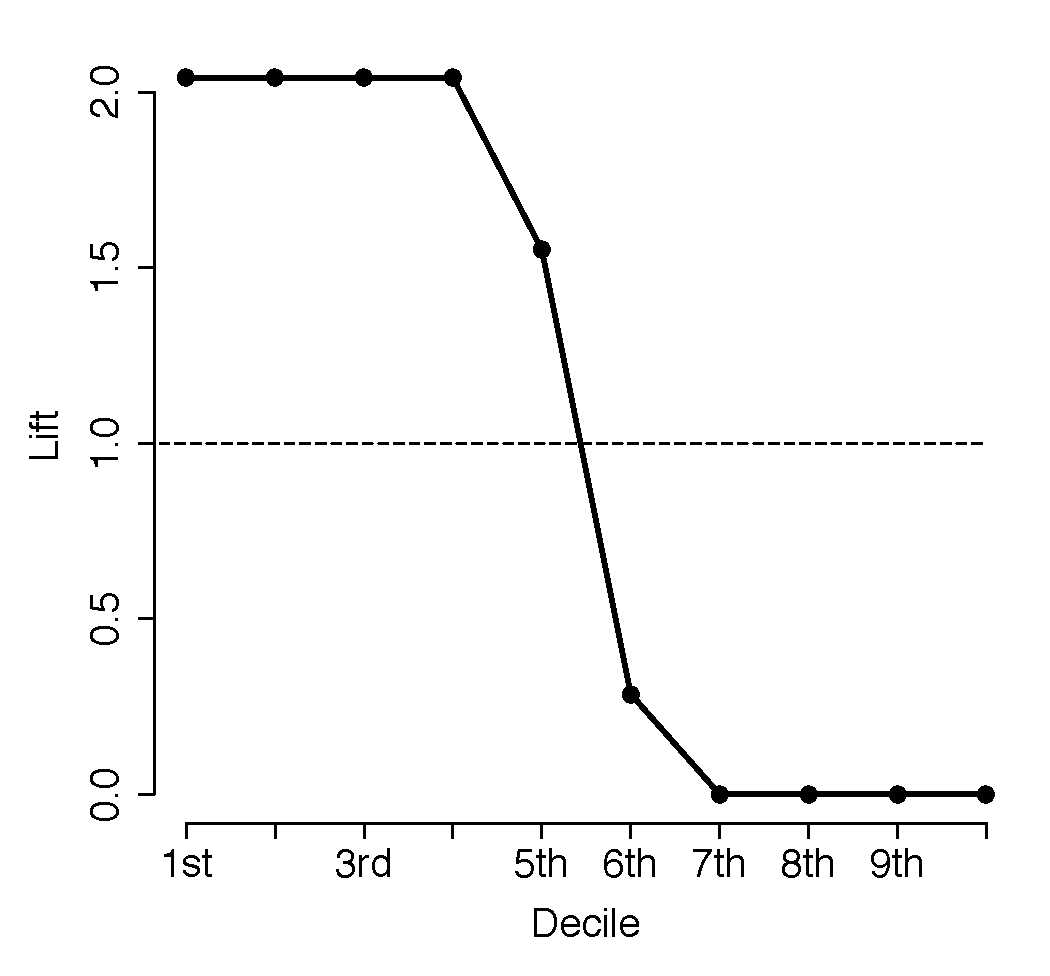
\includegraphics[width=0.24\textwidth]{images/Eval-LiftChart1.pdf}}
			\subfigure{\label{fig:bigLiftGainExamplesLift2}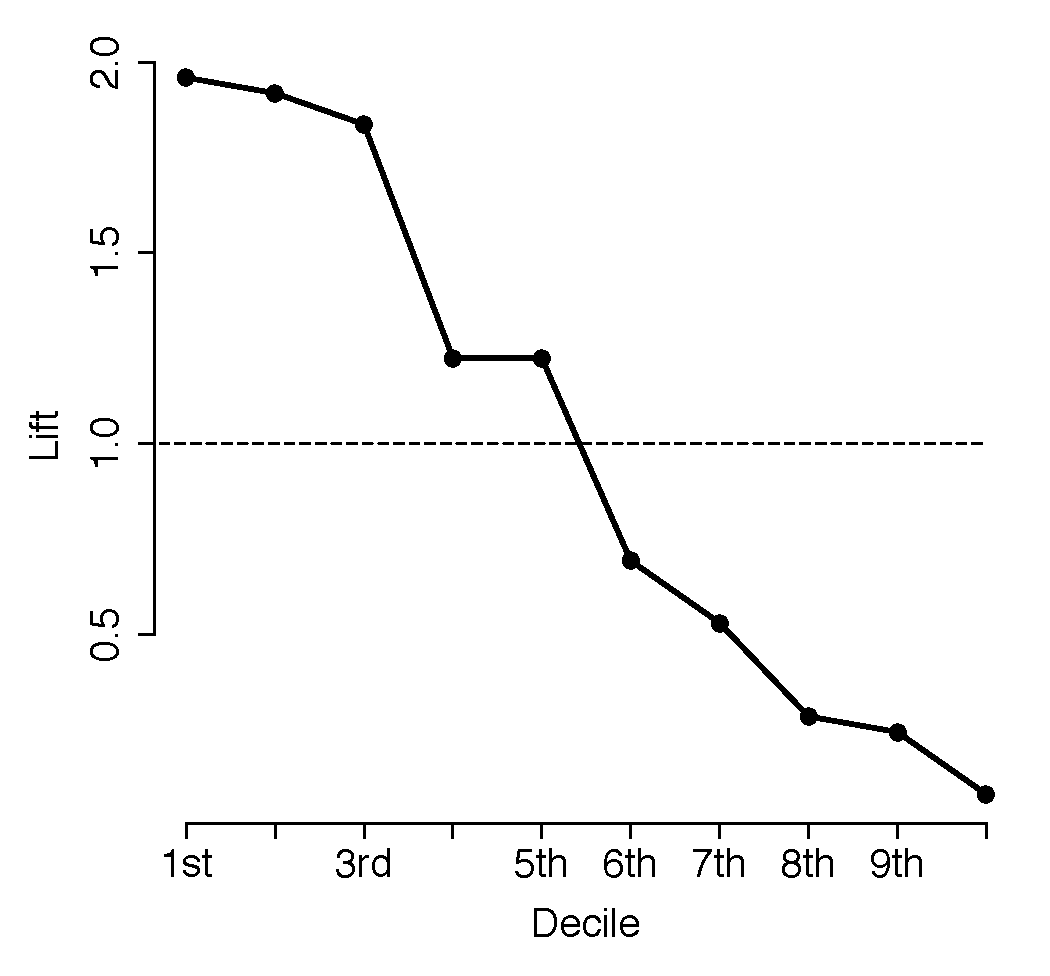
\includegraphics[width=0.24\textwidth]{images/Eval-LiftChart2.pdf}}
			\subfigure{\label{fig:bigLiftGainExamplesLift3}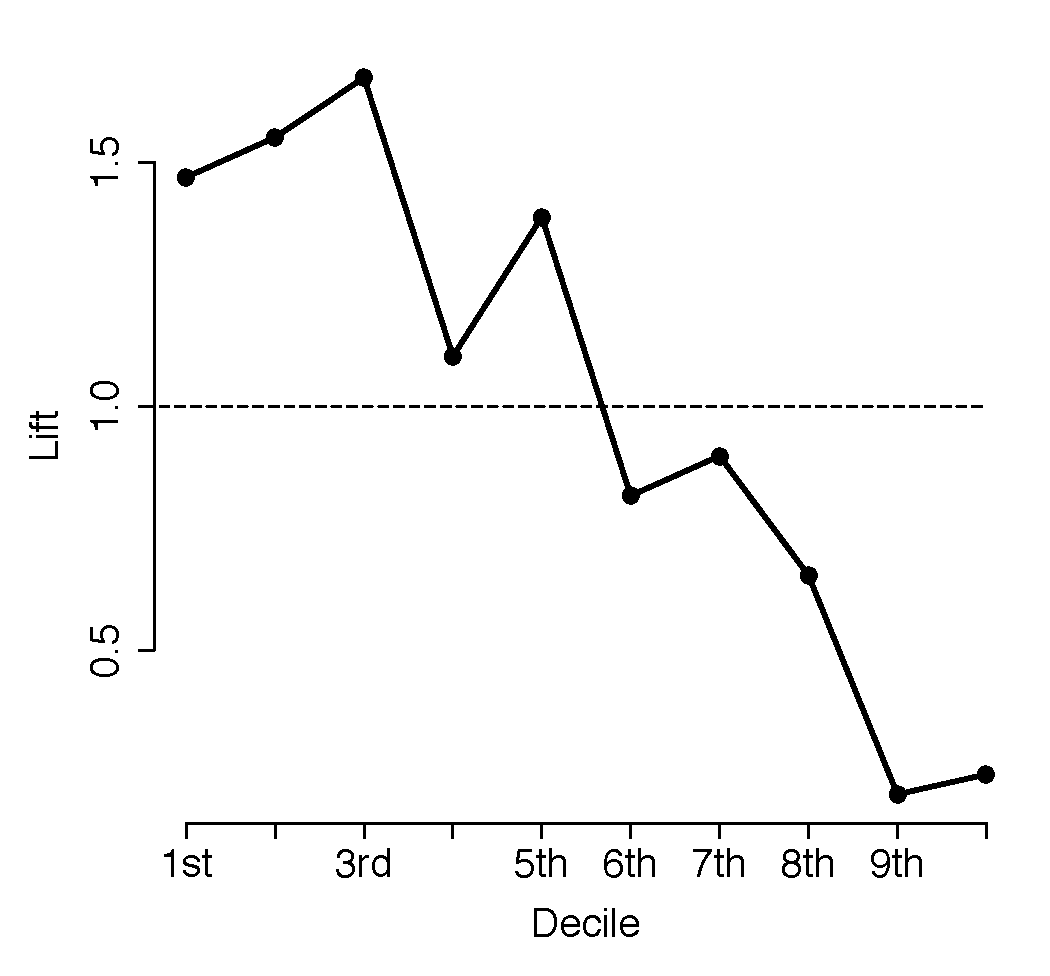
\includegraphics[width=0.24\textwidth]{images/Eval-LiftChart3.pdf}}		
			\subfigure{\label{fig:bigLiftGainExamplesLift4}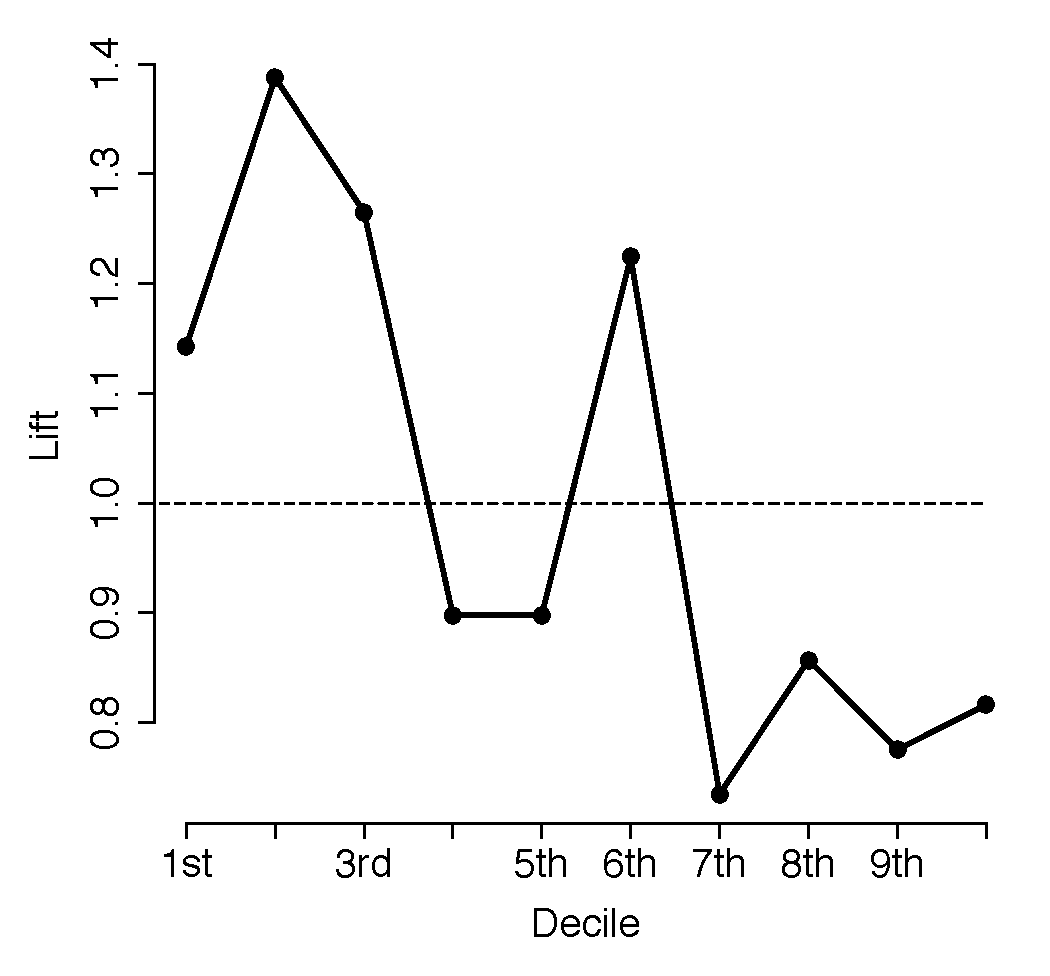
\includegraphics[width=0.24\textwidth]{images/Eval-LiftChart4.pdf}}			
			
			\subfigure{\label{fig:bigLiftGainExamplesCumLift1}\includegraphics[width=0.24\textwidth]{images/Eval-CumulativeLiftChart1.pdf}}
			\subfigure{\label{fig:bigLiftGainExamplesCumLift2}\includegraphics[width=0.24\textwidth]{images/Eval-CumulativeLiftChart2.pdf}}
			\subfigure{\label{fig:bigLiftGainExamplesCumLift3}\includegraphics[width=0.24\textwidth]{images/Eval-CumulativeLiftChart3.pdf}}
			\subfigure{\label{fig:bigLiftGainExamplesCumLift4}\includegraphics[width=0.24\textwidth]{images/Eval-CumulativeLiftChart4.pdf}}
			
       \caption{\indexkeyword{Cumulative gain}, \indexkeyword{lift}, and \indexkeyword{cumulative lift} charts for four different models for the extended email classification test set.}
       \label{fig:bigLiftGainExamples}
       \end{centering}
\end{figure}
\end{frame} 

\SectionSlideShortHeader{Performance Measures: Multinomial Targets}{Multinomial}

 \begin{frame} 
\begin{table}
\caption{The structure of a confusion matrix for a multinomial prediction problem with $l$ target levels.}
\label{tab:confusionMatrixStuctureMultiClass}
\centering
\begin{footnotesize}
\begin{tabular}{c >{\bfseries}r @{\hspace{0.7em}} | c @{\hspace{0.4em}} c @{\hspace{0.7em}} c @{\hspace{0.7em}} c @{\hspace{0.7em}} c @{\hspace{0.7em}} |  c @{\hspace{0.7em}}}
    & &  \multicolumn{5}{c|}{\bfseries Prediction}  & \multirow{2}{*}{ \bfseries Recall} \\
  & & \bfseries \textit{level1} & \bfseries \textit{level2} & \bfseries \textit{level3} & $\cdots$ & \bfseries \textit{levell} &  \\
  \hline
  \multirow{5}{*}{\parbox{1.1cm}{\bfseries\raggedleft Target}}  & \textit{level1} & - & - & - &  & - & - \\
  & \textit{level2} & - & - & - &  & -  & - \\
  & \textit{level3} & - & - & - &  & -  & - \\
  &  $\vdots$ &  &  &  & $\ddots$ &  & $\vdots$  \\
  & \textit{levell} & - & - & - &  & -  & - \\
  \hline
  & \bfseries Precision & - & - & - & $\cdots$ & -  &  \\
\end{tabular}
\end{footnotesize}
\end{table}
\end{frame} 



 \begin{frame} 
\begin{alignat}{2}
\text{precision(l)} & = \frac{TP(l)}{TP(l) + FP(l)} \label{eqn:precisionMulti}\\
\text{recall(l)} & = \frac{TP(l)}{TP(l) + FN(l)}  \label{eqn:recallMulti}
\end{alignat}
\end{frame} 



 \begin{frame} 
\begin{table}[htb]
	\caption{A sample test set with model predictions for a bacterial species identification problem.}
\label{tab:multinomialPredictionExample}
\centering
\begin{scriptsize}
\begin{tabular}{cc}
		\hline
			\begin{minipage}{0.36\textwidth}
					\begin{tabular}{ c c c }
\featN{ID}	 & Target	& Prediction \\
\hline
1	&	durionis	&	fructosus	\\
2	&	ficulneus	&	fructosus	\\
3	&	fructosus	&	fructosus	\\
4	&	ficulneus	&	ficulneus	\\
5	&	durionis	&	durionis	\\
6	&	pseudo.	&	pseudo.	\\
7	&	durionis	&	fructosus	\\
8	&	ficulneus	&	ficulneus	\\
9	&	pseudo.	&	pseudo.	\\
10	&	pseudo.	&	fructosus	\\
11	&	fructosus	&	fructosus	\\
12	&	ficulneus	&	ficulneus	\\
13	&	durionis	&	durionis	\\
14	&	fructosus	&	fructosus	\\
15	&	fructosus	&	ficulneus	\\
\hline 
\end{tabular}
			\end{minipage}
			&
			\begin{minipage}{0.36\textwidth}
										\begin{tabular}{ c c c }
\featN{ID}	 & Target	& Prediction \\
\hline
16	&	ficulneus	&	ficulneus	\\
17	&	ficulneus	&	ficulneus	\\
18	&	fructosus	&	fructosus	\\
19	&	durionis	&	durionis	\\
20	&	fructosus	&	fructosus	\\
21	&	fructosus	&	fructosus	\\
22	&	durionis	&	durionis	\\
23	&	fructosus	&	fructosus	\\
24	&	pseudo.	&	fructosus	\\
25	&	durionis	&	durionis	\\
26	&	pseudo.	&	pseudo.	\\
27	&	fructosus	&	fructosus	\\
28	&	ficulneus	&	ficulneus	\\
29	&	fructosus	&	fructosus	\\
30	&	fructosus	&	fructosus	\\
\hline 
\end{tabular}
			\end{minipage}\\
\end{tabular}
\end{scriptsize}
\end{table}
\end{frame} 

 \begin{frame} 
\begin{table}
\caption{A confusion matrix for a model trained on the bacterial species identification problem.}
\label{tab:confusionMatrixMultiClassExample}
\centering
\begin{scriptsize}
\begin{tabular}{c >{\bfseries}r @{\hspace{0.7em}} | c @{\hspace{0.4em}} c @{\hspace{0.7em}} c @{\hspace{0.7em}} c @{\hspace{0.7em}} |  c @{\hspace{0.7em}}}
    & &  \multicolumn{4}{c|}{\bfseries Prediction}  & \multirow{2}{*}{ \bfseries Recall} \\
  & & \bfseries \featL{durionis}	&	\bfseries \featL{ficulneus}	&	\bfseries \featL{fructosus}	&	\bfseries \featL{pseudo.} &  \\
  \hline
  \multirow{4}{*}{\parbox{1.1cm}{\bfseries\raggedleft Target}}  & \featL{durionis}	&	$5$	&	$0$	&	$2$	&	$0$	&	$0.714$ \\
  & \featL{ficulneus}	&	$0$	&	$6$	&	$1$	&	$0$	&	$0.857$ \\
  & \featL{fructosus}	&	$0$	&	$1$	&	$10$	&	$0$	&	$0.909$ \\
  & \featL{pseudo.}	&	$0$	&	$0$	&	$2$	&	$3$	&	$0.600$ \\
  \hline
  & \bfseries Precision &	$1.000$	&	$0.857$	&	$0.667$	&	$1.000$	&	 \\	
\end{tabular}
\end{scriptsize}
\end{table}
\end{frame} 

\begin{frame} 
\begin{itemize}
	\item The $\text{average class accuracy}_\text{HM}$ for this problem is:
\end{itemize}
\begin{alignat*}{2}
\displaystyle \frac{1}{\displaystyle  \frac{1}{4}\left(\frac{1}{0.714} + \frac{1}{0.857} + \frac{1}{0.909} + \frac{1}{0.600}\right)} = \frac{1}{1.333} = 75.000\%
\end{alignat*}
\end{frame} 


\SectionSlideShortHeader{Performance Measures: Continuous Targets}{Cont. Targets}

\subsection{Basic Measures of Error}

 \begin{frame} 
\begin{alignat}{2}
\text{sum of squared errors} = \frac{1}{2} \sum_{i=1}^{n} (t_i - \mathbb{M}(\mathbf{d}_i))^2 
\label{eq:sumOfSquaredErrors}
\end{alignat}
\begin{alignat}{2}
\text{mean squared error} =  \frac{\displaystyle\sum_{i=1}^{n} (t_i - \mathbb{M}(\mathbf{d}_i))^2}{n}
\label{eq:meanSquaredError}
\end{alignat}
\begin{alignat}{2}
\text{root mean squared error} =  \displaystyle \sqrt{\displaystyle \frac{ \displaystyle \sum_{i=1}^{n} (t_i - \mathbb{M}(\mathbf{d}_i))^2}{n}}
\label{eq:rootMeanSquaredError}
\end{alignat}
\begin{alignat}{2}
\text{mean absolute error} =  \displaystyle \frac{ \displaystyle \sum_{i=1}^{n} abs(t_i - \mathbb{M}(\mathbf{d}_i))}{n}
\label{eq:meanAbsolouteError}
\end{alignat}
\end{frame} 



 \begin{frame} [plain]
\begin{table}[!bht]
%\caption{The expected target values for a test set, the predictions made by a model, and the resulting errors based on these predictions for a blood thinning drug dosage prediction problem.}
\label{tab:continuousPredictionDataset}
\centering
\begin{tiny}
\begin{tabular}{ c r r r r r }
\hline
	 & 	& \multicolumn{2}{c}{Linear Regression} & \multicolumn{2}{c}{$k$-NN} \\
\featN{ID}	 & Target	& Prediction & Error & Prediction & Error\\
\hline
1	&	10.502	&	10.730	&	0.228	&	12.240	&	1.738	\\
2	&	18.990	&	17.578	&	-1.412	&	21.000	&	2.010	\\
3	&	20.000	&	21.760	&	1.760	&	16.973	&	-3.027	\\
4	&	6.883	&	7.001	&	0.118	&	7.543	&	0.660	\\
5	&	5.351	&	5.244	&	-0.107	&	8.383	&	3.032	\\
6	&	11.120	&	10.842	&	-0.278	&	10.228	&	-0.892	\\
7	&	11.420	&	10.913	&	-0.507	&	12.921	&	1.500	\\
8	&	4.836	&	7.401	&	2.565	&	7.588	&	2.752	\\
9	&	8.177	&	8.227	&	0.050	&	9.277	&	1.100	\\
10	&	19.009	&	16.667	&	-2.341	&	21.000	&	1.991	\\
11	&	13.282	&	14.424	&	1.142	&	15.496	&	2.214	\\
12	&	8.689	&	9.874	&	1.185	&	5.724	&	-2.965	\\
13	&	18.050	&	19.503	&	1.453	&	16.449	&	-1.601	\\
14	&	5.388	&	7.020	&	1.632	&	6.640	&	1.252	\\
15	&	10.646	&	10.358	&	-0.288	&	5.840	&	-4.805	\\
16	&	19.612	&	16.219	&	-3.393	&	18.965	&	-0.646	\\
17	&	10.576	&	10.680	&	0.104	&	8.941	&	-1.634	\\
18	&	12.934	&	14.337	&	1.403	&	12.484	&	-0.451	\\
19	&	10.492	&	10.366	&	-0.126	&	13.021	&	2.529	\\
20	&	13.439	&	14.035	&	0.596	&	10.920	&	-2.519	\\
21	&	9.849	&	9.821	&	-0.029	&	9.920	&	0.071	\\
22	&	18.045	&	16.639	&	-1.406	&	18.526	&	0.482	\\
23	&	6.413	&	7.225	&	0.813	&	7.719	&	1.307	\\
24	&	9.522	&	9.565	&	0.043	&	8.934	&	-0.588	\\
25	&	12.083	&	13.048	&	0.965	&	11.241	&	-0.842	\\
26	&	10.104	&	10.085	&	-0.020	&	10.010	&	-0.095	\\
27	&	8.924	&	9.048	&	0.124	&	8.157	&	-0.767	\\
28	&	10.636	&	10.876	&	0.239	&	13.409	&	2.773	\\
29	&	5.457	&	4.080	&	-1.376	&	9.684	&	4.228	\\
30	&	3.538	&	7.090	&	3.551	&	5.553	&	2.014	\\
\hline 
\multicolumn{2}{r}{\textbf{MSE}} &  \multicolumn{2}{r}{$\textbf{1.905}$} &   \multicolumn{2}{r}{$\textbf{4.394}$} \\
\multicolumn{2}{r}{\textbf{RMSE}} &  \multicolumn{2}{r}{$\textbf{1.380}$} &   \multicolumn{2}{r}{$\textbf{2.096}$} \\
\multicolumn{2}{r}{\textbf{MAE}} &  \multicolumn{2}{r}{$\textbf{0.975}$} &   \multicolumn{2}{r}{$\textbf{1.750}$} \\
\multicolumn{2}{r}{\textbf{$R^2$}} &  \multicolumn{2}{r}{$\textbf{0.889}$} &   \multicolumn{2}{r}{$\textbf{0.776}$} \\
\hline
\end{tabular}
\end{tiny}
\end{table}
\end{frame} 

\subsection{Domain Independent Measures of Error}

 \begin{frame} 
\begin{alignat}{2}
R^2 = 1 - \frac{\text{sum of squared errors}}{\text{total sum of squares}}  \label{eqn:rSquaredEval}
\end{alignat}
\begin{alignat}{2}
\text{total sum of squares} = \frac{1}{2}\sum_{i=1}^{n} \left( t_i - \overline{t} \right)^2 \label{eqn:sstEval}
\end{alignat}
\end{frame} 


\SectionSlideShortHeader{Evaluating Models after Deployment}{Deployment}

\begin{frame}
\noindent To monitor the on-going performance of a model, we need a signal that indicates that something has changed. There are three sources from which we can extract such a signal:
\begin{enumerate}
	\item The performance of the model measured using appropriate performance measures
	\item The distributions of the outputs of a model
	\item The distributions of the descriptive features in query instances presented to the model
\end{enumerate}
\end{frame}

\subsection{Monitoring Changes in Performance Measures}

\begin{frame}
\begin{itemize}
	\item The simplest way to get a signal that concept drift has occurred is to repeatedly evaluate models with the same performance measures used to evaluate them before deployment. 
	\item We can calculate performance measures for a deployed model and compare these to the performance achieved in evaluations before the model was deployed. 
	\item If the performance changes significantly, this is a strong indication that \keyword{concept drift} has occurred and that the model has gone stale.
\end{itemize}
\end{frame}

\begin{frame}
	\begin{itemize}
		\item Although monitoring changes in the performance of a model is the easiest way to tell whether it has gone stale, this method makes the rather large assumption that the correct target feature value for a query instance will be made available shortly after the query has been presented to a deployed model.
	\end{itemize}
\end{frame}

\subsection{Monitoring Model Output Distributions}

 \begin{frame} 
  \begin{itemize}
 	\item An alternative to using changing model performance is to use changes in the distribution of model outputs as a signal for concept drift.
\end{itemize}
\begin{footnotesize}
\begin{equation}
\text{stability index}=\sum_{l\in levels(t)} \left(\left(\frac{|\mathcal{A}_{t=l}|}{|\mathcal{A}|} - \frac{|\mathcal{B}_{t=l}|}{|\mathcal{B}|}\right) \times log_e\left(\displaystyle \frac{|\mathcal{A}_{t=l}|}{|\mathcal{A}|} / \frac{|\mathcal{B}_{t=l}|}{|\mathcal{B}|}\right)\right)
\label{eq:stabilityIndex}
\end{equation}
\end{footnotesize}
\end{frame} 

\begin{frame}
In general,
\begin{itemize}
	\item stability index $<0.1$, then the distribution of the newly collected test set is broadly similar to the distribution in the original test set.
	\item stability index is between $0.1$ and $0.25$, then some change has occurred and further investigation may be useful.
	\item stability index $>0.25$ suggests that a significant change has occurred and corrective action is required. 
\end{itemize}
\end{frame}

 \begin{frame} [plain]
\begin{table}
	\caption{Calculating the \indexkeyword{stability index} for the bacterial species identification problem given new test data for two periods after model deployment. The frequency and percentage of each target level are shown for the original test set and for two samples collected after deployment. The column marked SI$_t$ shows the different parts of the stability index sum based on Equation \ourEqRef{eq:stabilityIndex}.}
\label{tab:stabilityIndexExample}
\centering
	\begin{scriptsize}
		\begin{tabular}[ht]{r c c c c c c c c}  
				\hline
	&	\multicolumn{2}{c}{Original}		&	\multicolumn{3}{c}{New Sample 1}		&	\multicolumn{3}{c}{New Sample 2}	\\
Target & Count	&	\%	&	Count	&	\%	&	SI$_t$	&	Count	&	\%	&	SI$_t$	\\
				\hline
\featL{durionis}	&	$7$	&	$0.233$	&	$12$	&	$0.267$	&	$0.004$	&	$12$	&	$0.200$	&	$0.005$	\\
\featL{ficulneus}	&	$7$	&	$0.233$	&	$8$	&	$0.178$	&	$0.015$	&	$9$	&	$0.150$	&	$0.037$	\\
\featL{fructosus}	&	$11$	&	$0.367$	&	$16$	&	$0.356$	&	$0.000$	&	$14$	&	$0.233$	&	$0.060$	\\
\featL{pseudo.}	&	$5$	&	$0.167$	&	$9$	&	$0.200$	&	$0.006$	&	$25$	&	$0.417$	&	$0.229$	\\
				\hline
\textbf{Sum}	&	$30$	&		&	$45$	&		&	$\textbf{0.026}$ 	&	$60$	&		&	$\textbf{0.331}$	\\
				\hline
			\end{tabular}
			\end{scriptsize}
\end{table}
\end{frame} 



 \begin{frame} 
\begin{eqnarray*}
\text{stability index} & = & ~~\left(\frac{7}{30} - \frac{12}{45}\right) \times log_e\left( \frac{7}{30} /  \frac{12}{45}\right) \\
&  & + \left(\frac{7}{30} - \frac{8}{45}\right) \times log_e\left( \frac{7}{30} /  \frac{8}{45}\right) \\
&  & + \left(\frac{11}{30} - \frac{16}{45}\right) \times log_e\left( \frac{11}{30} /  \frac{16}{45}\right) \\
&  & + \left(\frac{5}{30} - \frac{9}{45}\right) \times log_e\left( \frac{5}{30} /  \frac{9}{45}\right) \\
& = & 0.026
\end{eqnarray*}
\end{frame} 

 \begin{frame} [plain]
\begin{figure}[htb]
       \begin{centering}
			\subfigure[Original]{\label{fig:stabilityIndexPlotsOriginal}\includegraphics[width=0.35\textwidth]{images/Eval-StabilityIndexOriginal.pdf}}
			\subfigure[New Sample 1]{\label{fig:stabilityIndexPlotsOngoing1}\includegraphics[width=0.35\textwidth]{images/Eval-StabilityIndexOngoing1.pdf}}
			\subfigure[New Sample 2]{\label{fig:stabilityIndexPlotsOngoing2}\includegraphics[width=0.35\textwidth]{images/Eval-StabilityIndexOngoing2.pdf}}
						\subfigure[Monitoring Over Time]{\label{fig:stabilityIndexPlotsOverTime}\includegraphics[width=0.35\textwidth]{images/Eval-StabilityIndexOverTime.pdf}}
       \caption{The distributions of predictions made by a model trained for the bacterial species identification problem for (a) the original evaluation test set and for (b) and (c) two periods of time after model deployment; (d) shows how the stability index should be tracked over time to monitor for concept drift.}
       \label{fig:stabilityIndexPlots}
       \end{centering}
\end{figure}
\end{frame} 

\subsection{Monitoring Descriptive Feature Distribution Changes}

\begin{frame}
	\begin{itemize}
		\item In the same way we can compare the distributions of model outputs between the time that the model was built and after deployment, we can also make the same type of comparison for the distributions of the descriptive features used by the model.  
		\item We can use any appropriate measure that captures the difference between two different distributions for this, including the stability index, the \indexkeyword{$\chi^2$ statistic}, and the \alert{K-S statistic}. 
	\end{itemize}
\end{frame}

\begin{frame}
	\begin{itemize}
		\item There is, however, a challenge here, as usually, there are a large number of descriptive features for which measures need to be calculated and tracked. 
		\item Furthermore, it is unlikely that a change in the distribution of just one descriptive feature in a multi-feature model will have a large impact on model performance. 
		\item For this reason, unless a model uses a very small number of descriptive features  (generally fewer than $10$), we do not recommend this approach.
	\end{itemize}
\end{frame}

\subsection{Comparative Experiments Using a Control Group}

\begin{frame}
	\begin{itemize}
		\item We use control groups not to evaluate the predictive power of the models themselves, but rather to evaluate how good they are at helping with the business problem when they are deployed.
	\end{itemize}
\end{frame}

 \begin{frame} [plain]
\begin{table}
	\caption{The number of customers who left the mobile phone network operator each week during the comparative experiment from both the control group (random selection) and the treatment group (model selection).}
\label{tab:controlGroupExample}
	\centering
	\begin{footnotesize}
		\begin{tabular}[ht]{c c c}  
				\hline
					&	Control Group	&	Treatment Group	\\
				Week	&	(Random Selection)	&	(Model Selection)	\\
				\hline
1	&	21	&	23	\\
2	&	18	&	15	\\
3	&	28	&	18	\\
4	&	19	&	20	\\
5	&	18	&	15	\\
6	&	17	&	17	\\
7	&	23	&	18	\\
8	&	24	&	20	\\
9	&	19	&	18	\\
10	&	20	&	19	\\
11	&	18	&	13	\\
12	&	21	&	16	\\
				\hline
\textbf{Mean}		& 	20.500	&	17.667 \\
\textbf{Std. Dev.}		& 3.177		&	2.708 \\
				\hline
			\end{tabular}
				\end{footnotesize}
\end{table}
\end{frame} 

\begin{frame}
	\begin{itemize}
		\item These figures show that, on average, fewer customers churn when the churn prediction model is used to select which customers to call.
	\end{itemize}
\end{frame}

\SectionSlideShortHeader{Summary}{Sum.}

\begin{frame}[plain]
	\begin{scriptsize}
	\vspace{0.25cm}
	\tableofcontents
	\end{scriptsize}
\end{frame}

\end{document}
